\section{Double weights} \label{sec:DW}

Throughout LHC Runs 1 and 2, the on-detector ECAL FENIX chip, a custom ASIC, was used for energy reconstruction to form $E_{T}$ sums for ECAL TPs, multiplying one set of weights by recorded digis as described in Section \ref{sec:ECAL_TP}. During LS2, it was discovered that the ECAL FENIX chip has the capacity to store and use two sets of weights. This essentially duplicates the ECAL FENIX data path, as shown in Figure \ref{fig:DW_Diagram}, into two electronically equivalent paths, one for each FIR filter named the ``EVEN" and ``ODD" filters.

\begin{figure}[H]
    \centering
    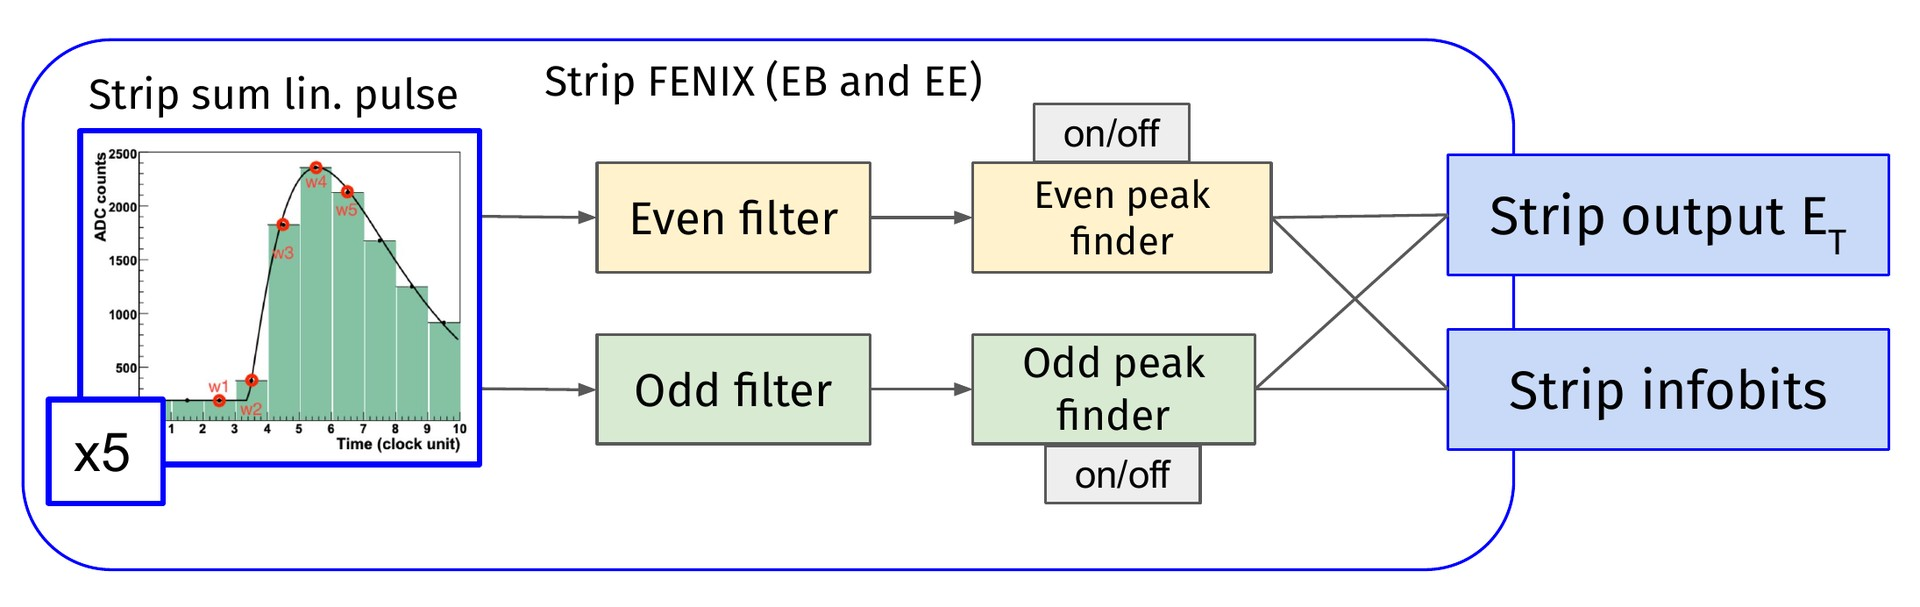
\includegraphics[width=\textwidth]{Images/ECAL/DW/ECAL_DW_Schematic.png}
    \caption{ECAL double weights mechanism.}
    \label{fig:DW_Diagram}
\end{figure}

This feature was implemented in the ECAL FENIX chip for potential further use, but was never used during Runs 1 and 2. 

\subsection{Spikes} \label{sec:spikes}

A commonly observed phenomenon at the ECAL is the direct ionization of the ECAL EB APDs, which produce anomalous signals termed ``spikes". Because these signals do not come from electromagnetic showers originating from the hard interactions of LHC collisions, they must be removed as efficiently as possible to keep trigger rates under control and preserve the quality of the offline reconstruction of electrons, photons and jets. Additionally, spike progenitors often spend time propagating in the CMS detector before directly ionizing the EB APDs, and therefore may be out-of-time with respect to electromagnetic signals.

There is a method in place used to remove spikes at L1 using a topological cut, termed the ``spike killer" \cite{Petyt_2012}. This operates by making a topological cut, exploiting the fact that spikes typically deposit all of their energy into a single ECAL crystal as they are due to the direct ionization of APDs, while EM showers are expected to be spread among multiple crystals. A diagram showing the mechanism of the spike killer is shown in Figure \ref{fig:spikeKillerDiagram}. 

\begin{figure}[H]
    \centering
    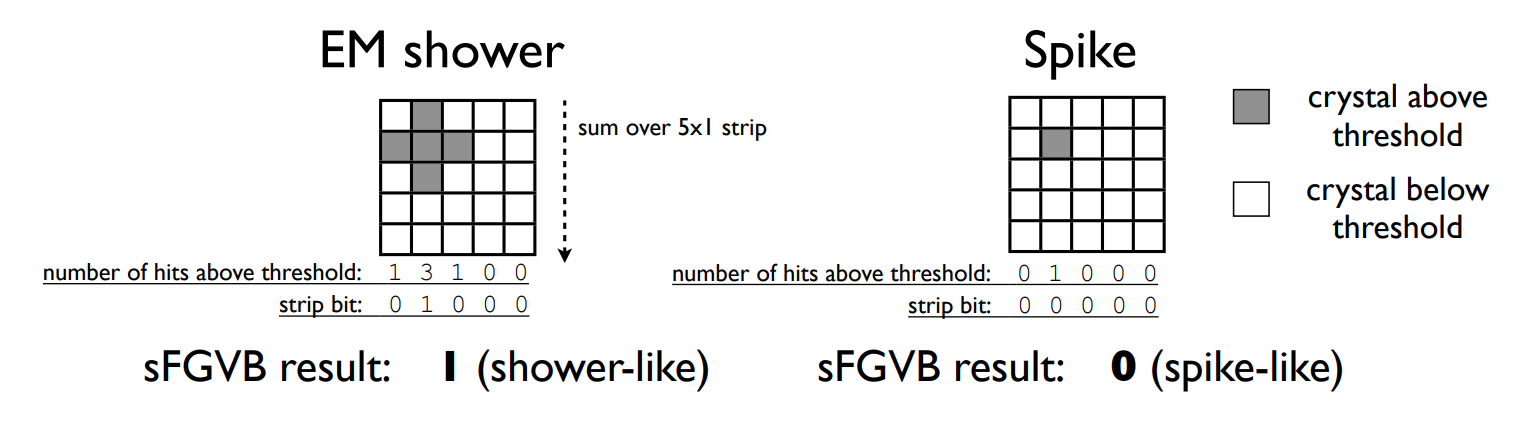
\includegraphics[width=\textwidth]{Images/ECAL/DW/SpikeKillerDiagram.png}
    \caption{Operation of the strip Fine-Grained Veto Bit (sFGVB) on an electromagnetic shower (left) and a spike-like energy deposit (right).}
    \label{fig:spikeKillerDiagram}
\end{figure}

The spike killer makes use of a per-strip bit, the strip Fine-Grained Veto Bit (sFGVB) which is set to 1 if at least 2 crystals in a strip are above a per-crystal energy threshold. If a trigger tower (set of 25 crystals, 5 strips) has at least one strip with a sFGVB equal to 1, it is preserved as it is considered EM shower-like due to its spread in energy. However, if a TT has no strips with at least one sFGVB set to 1, the TP energy is set to 0 if its energy is above the spike killer ``killing threshold" of 16 GeV. 

In order to optimize the spike killer for Run 3 where higher noise and everage PU is expected, the per-crystal energy threshold was increased, as there will be a higher expected contribution from noise and PU for all crystals. The spike contamination among TPs with the Run 2, and candidate Run 3 working point is shown in Figure \ref{fig:spikeKillerRun3optimization}. Notably in this spike contamination plot, produced using data from a ZeroBias dataset (no triggering on typical physics menus), there is a high spike contamination at high energy. This is because it is more likely to produce a high energy spike, which are high energy due to its direct ionization of the APDs, than a high energy EM shower, which requires the production of a truly high energy particle from proton-proton interactions. 

\begin{figure}[H]
    \centering
    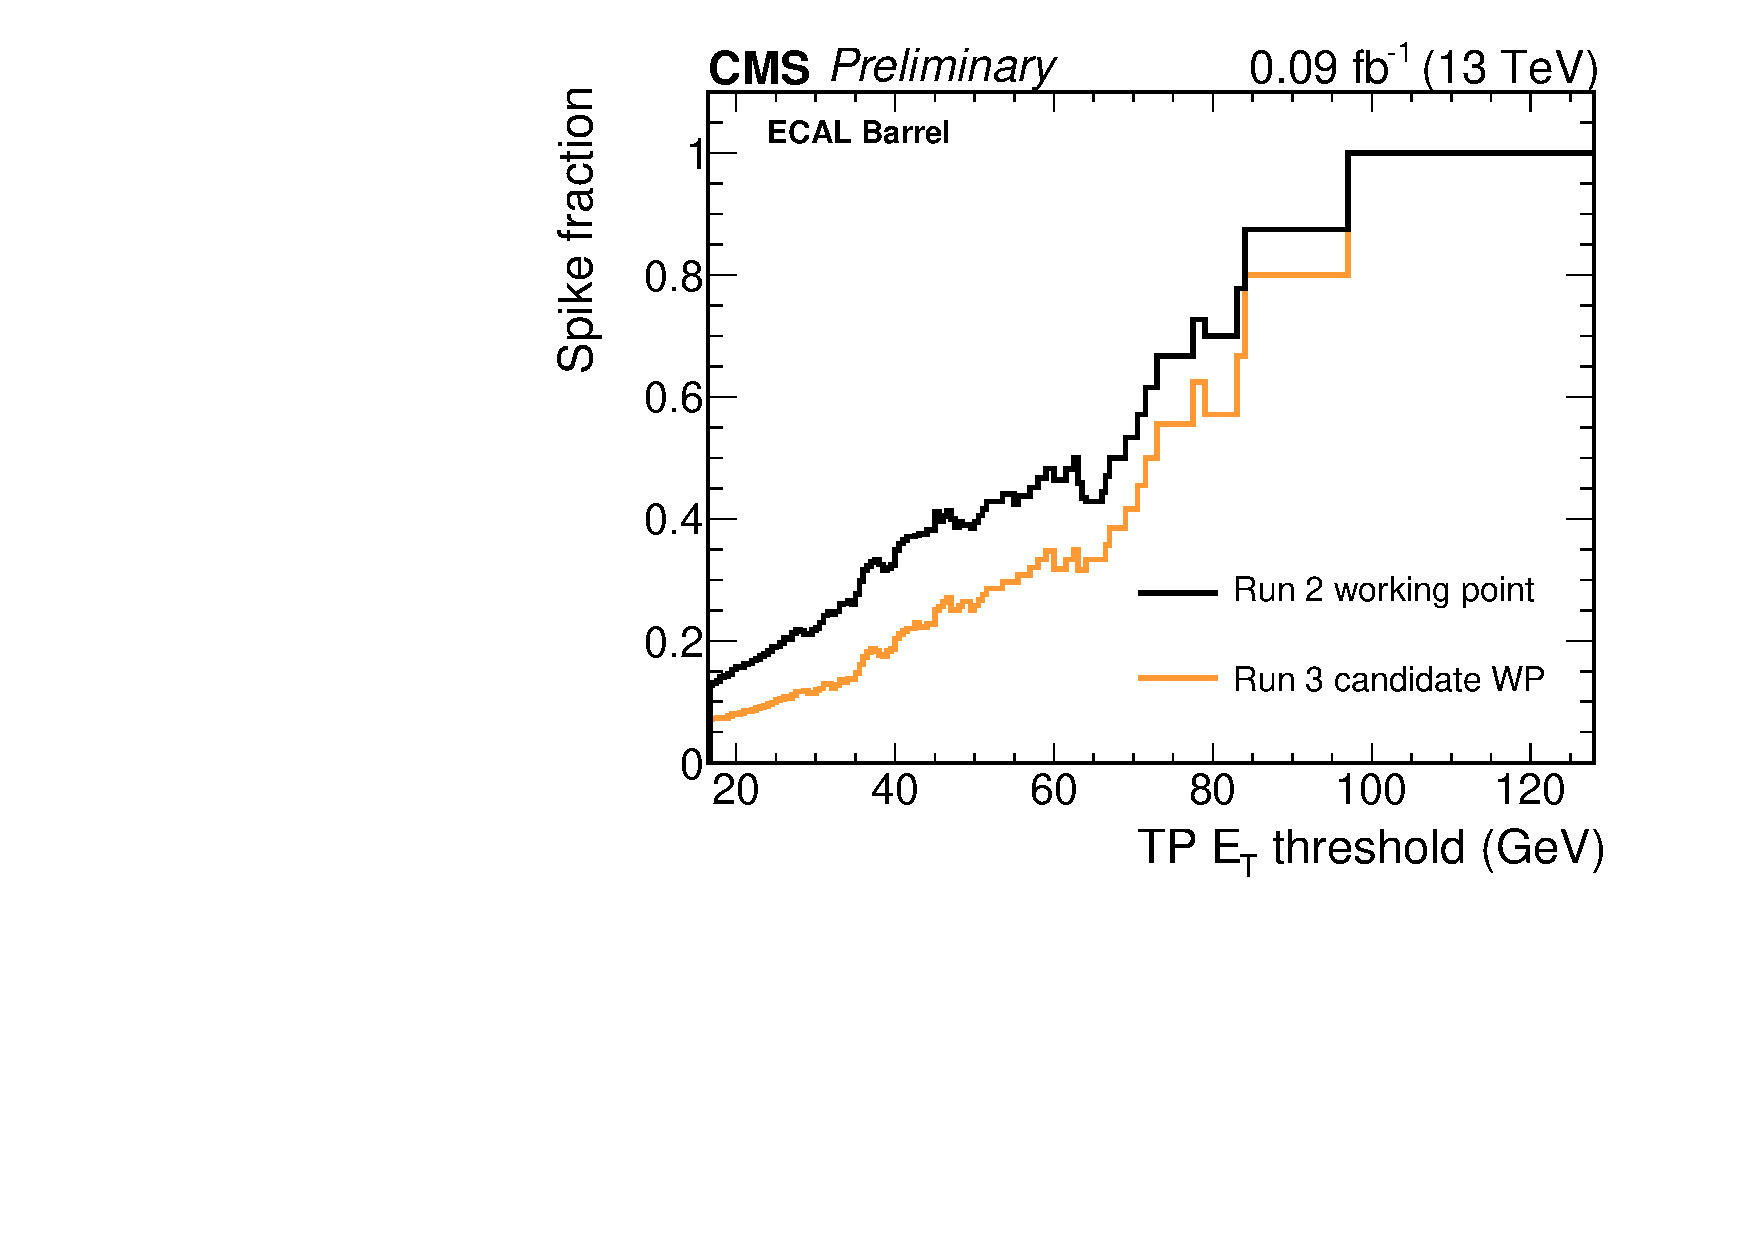
\includegraphics[width=0.8\textwidth]{Images/ECAL/DW/spikekiller_run3_optimisation.pdf}
    \caption{Spike fraction vs. TP $E_{T}$ threshold with a Run 2, and Run 3 candidate working point of the existing ECAL L1 spike killer. The data comes from a ZeroBias dataset recorded in July 2018 with a peak pileup of 50.}
    \label{fig:spikeKillerRun3optimization}
\end{figure}

This shows that while updating the settings of the existing spike killer to a candidate Run 3 working point removes additional spikes at Level-1, there is much room for improvement, especially in the high energy regime. Additionally, at L1 there is no existing spike killer in the low energy regime 0-16 GeV, as this is below the spike killer threshold. 

\subsection{Timing weights}

The initial idea for optimizing ECAL double weights was to keep the original set of amplitude weights in the EVEN filter, and to utilize the second set of weights, the ODD filter, as a set of timing weights in order to compute an on-detector timing value for trigger primitives. These studies showed possible discrimination power, as the timing weights were able to identify out of time signals which came from spikes. Figures \ref{fig:ampvstime_EMlike} and \ref{fig:ampvstime_Spikelike} show the reconstructed amplitude computed as the EVEN weights times signal digis, vs. the reconstructed time as computed by multiplying a set of optimal timing weights occupying the ODD filter by signal digis for signal and spike-like TPs in CMS data. 

\begin{figure}[H]
    \centering
    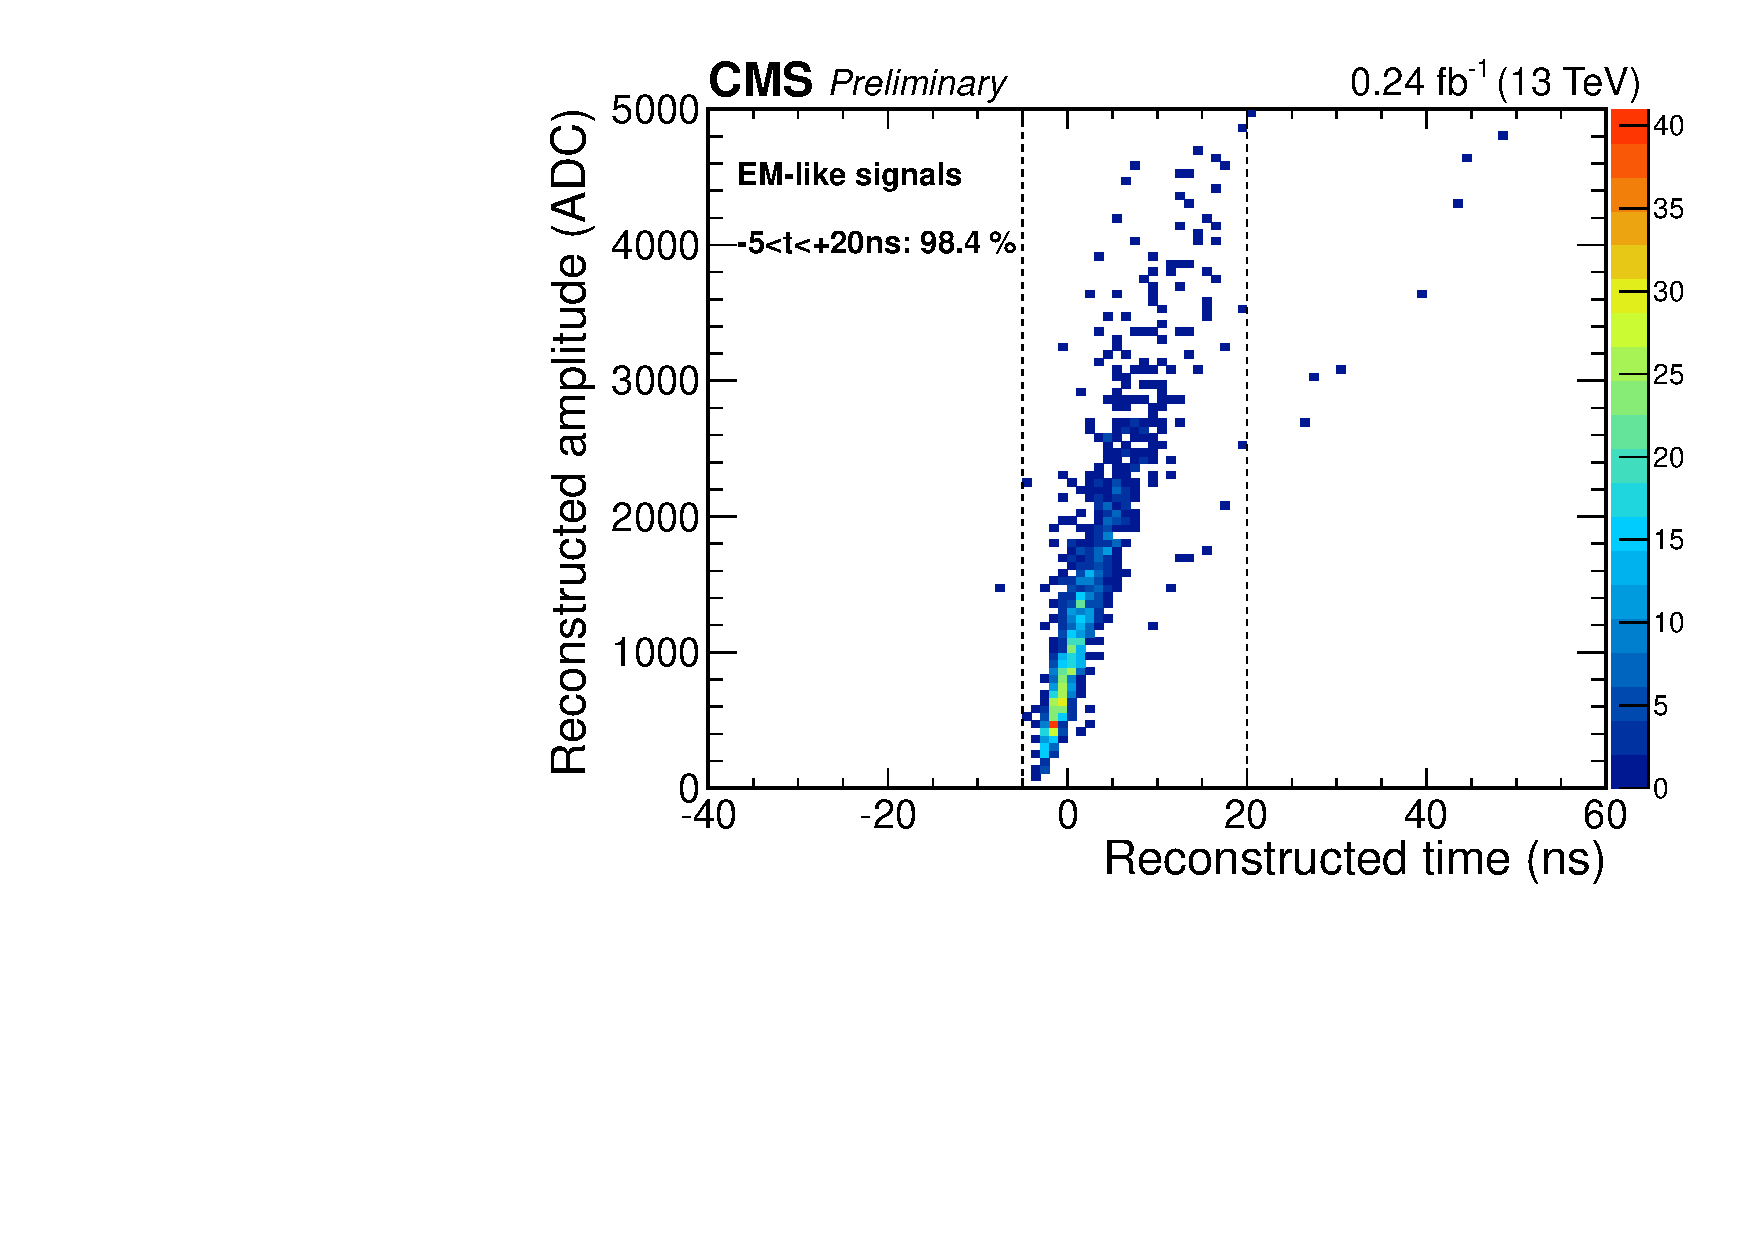
\includegraphics[width=0.8\textwidth]{Images/ECAL/DW/EM_TPs.pdf}
    \caption{Reco amplitude vs. Reco time of EM-like signals in CMS data}
    \label{fig:ampvstime_EMlike}
\end{figure}

\begin{figure}[H]
    \centering
    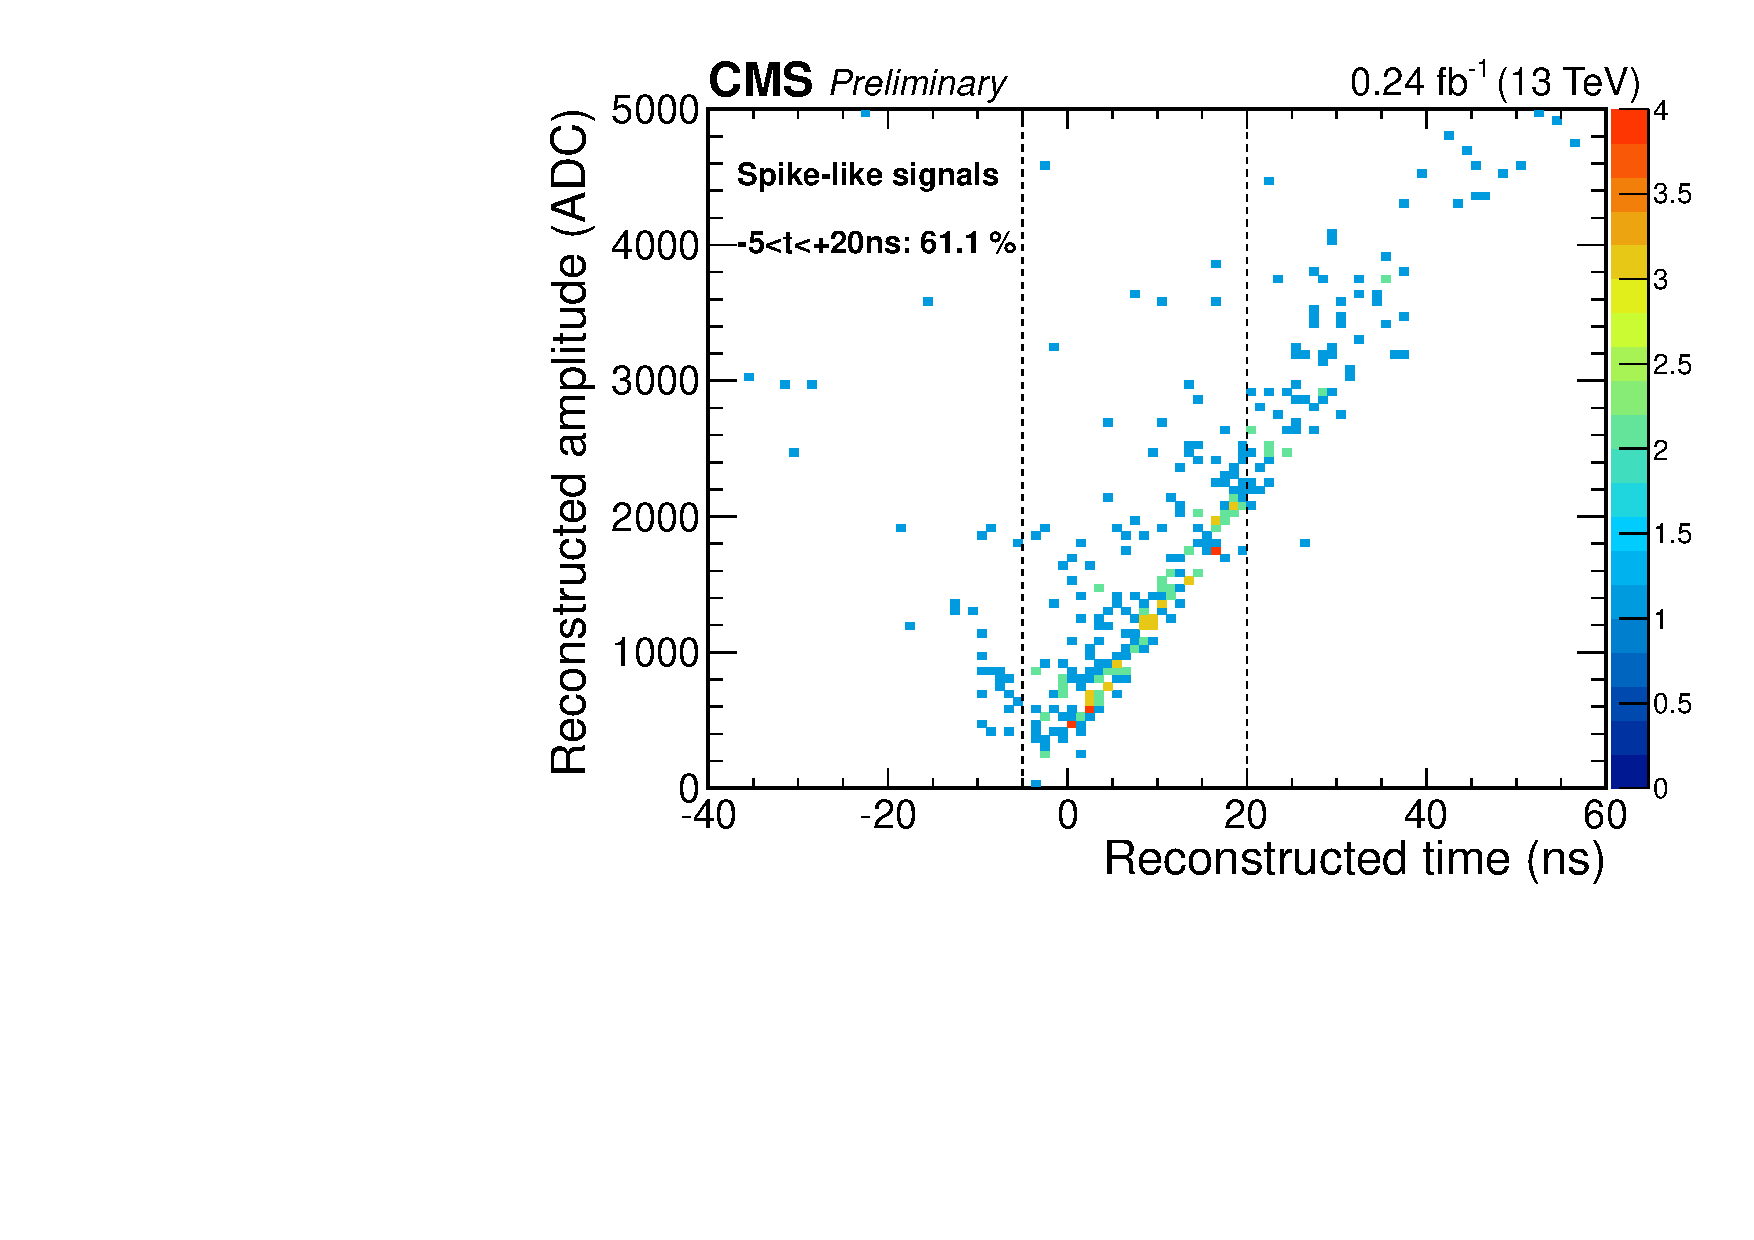
\includegraphics[width=0.8\textwidth]{Images/ECAL/DW/Spike_TPs.pdf}
    \caption{Reco amplitude vs. Reco time of spike-like signals in CMS data}
    \label{fig:ampvstime_Spikelike}
\end{figure}

By eye, most EM-like signals fall within a reconstructed time window near zero, with a tail going out to around 20 ns for signals with a greater reconstructed amplitude. For spike-like signals, there is a larger time window with some TPs very out-of-time. Interestingly, in the EM-like signals on Figure \ref{fig:ampvstime_EMlike} one can see a low population line of entries which appears to follow the trend of the spike-like signals in Figure \ref{fig:ampvstime_Spikelike}, as these are possibly real spikes which are incorrectly tagged offline as signal-like. 

For the sake of quantifying the possible discrimination power of ECAL timing weights, a hypothetical timing cut of -5 $<$ t $<$ 20 ns would have been able to drastically reduce the rate of spikes, as shown in Figure \ref{fig:TimingCutSpikeReduction}.

\begin{figure}[H]%
    \setcounter{subfigure}{0} % reset subcaption counter to 0 (a) 
    \centering
    \subfloat[Spike Rates]{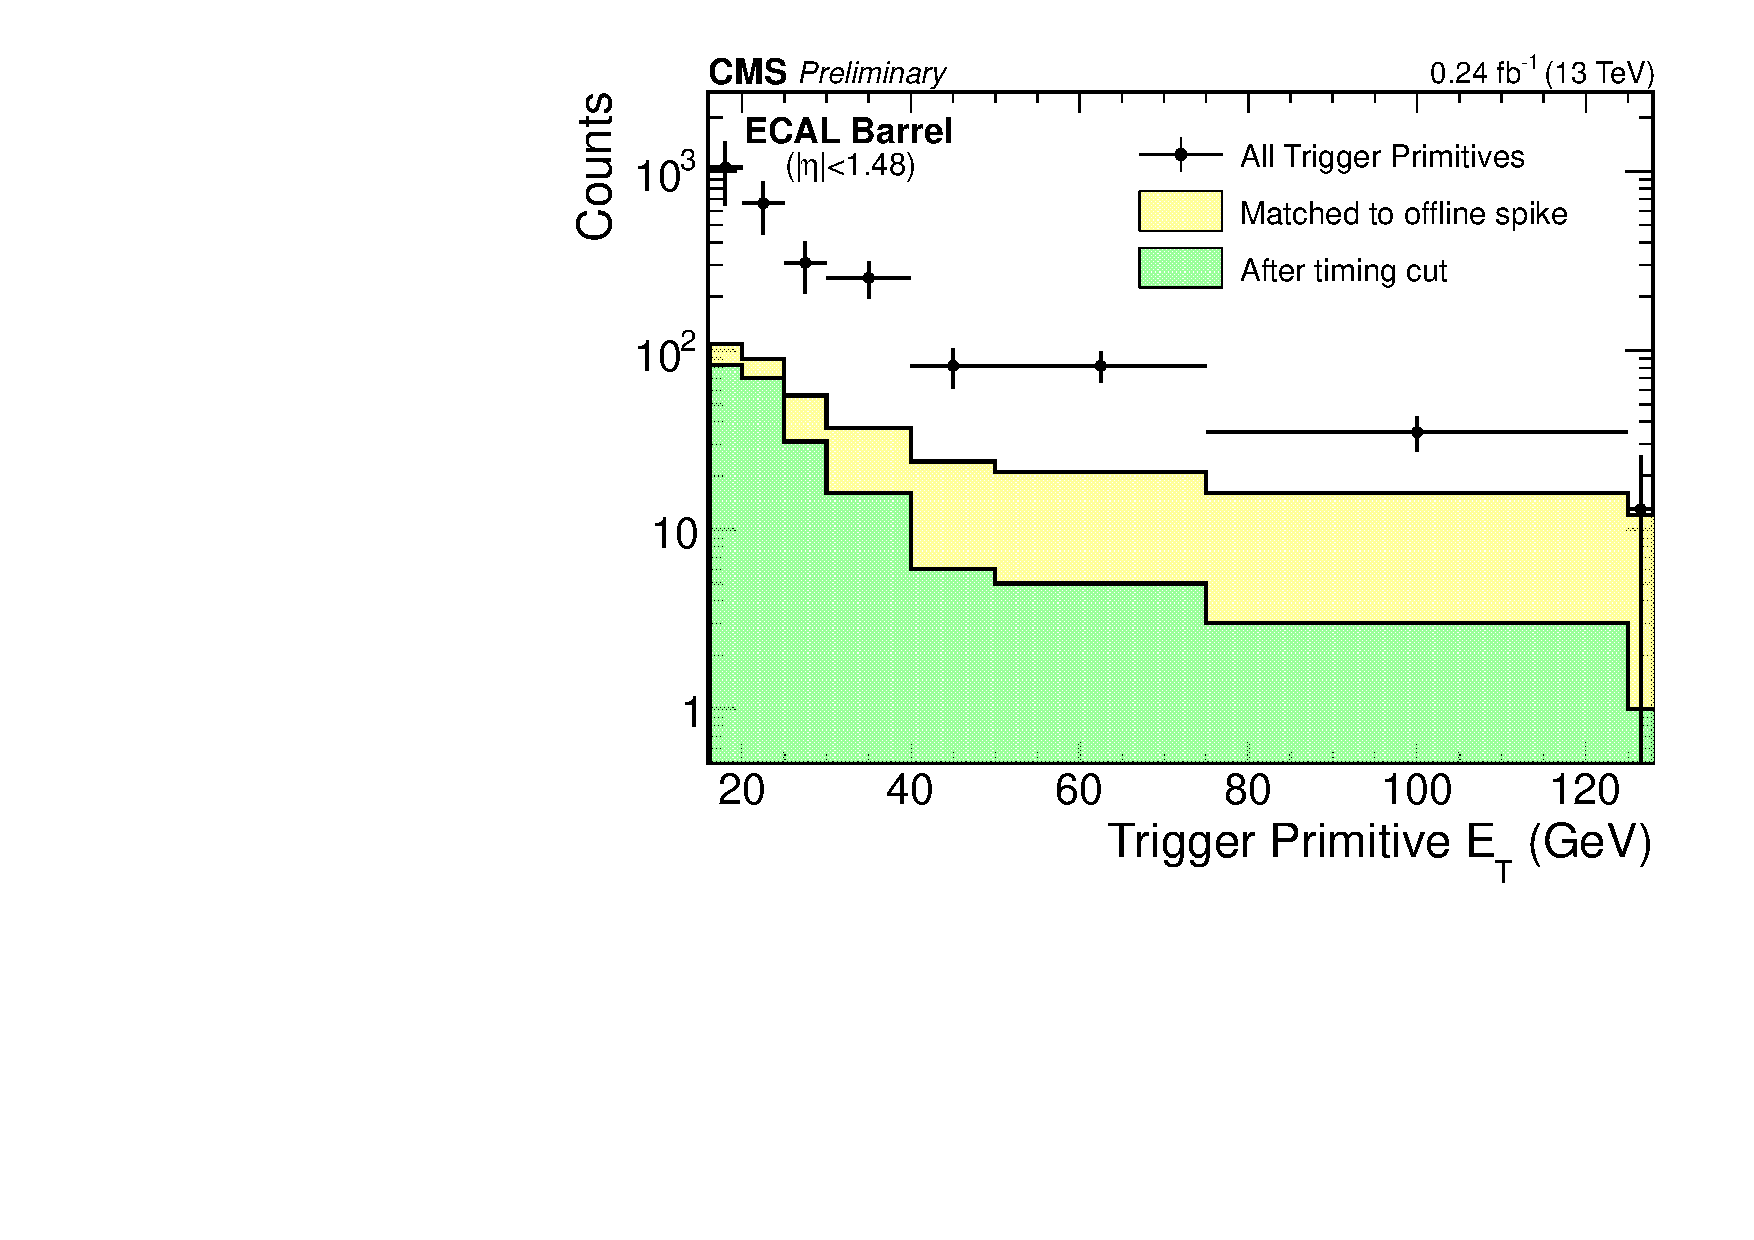
\includegraphics[width=0.49\textwidth]{Images/ECAL/DW/spikeTPet_beforeaftertimingcut.pdf}}%
    %\qquad
    \subfloat[Spike Fractions]{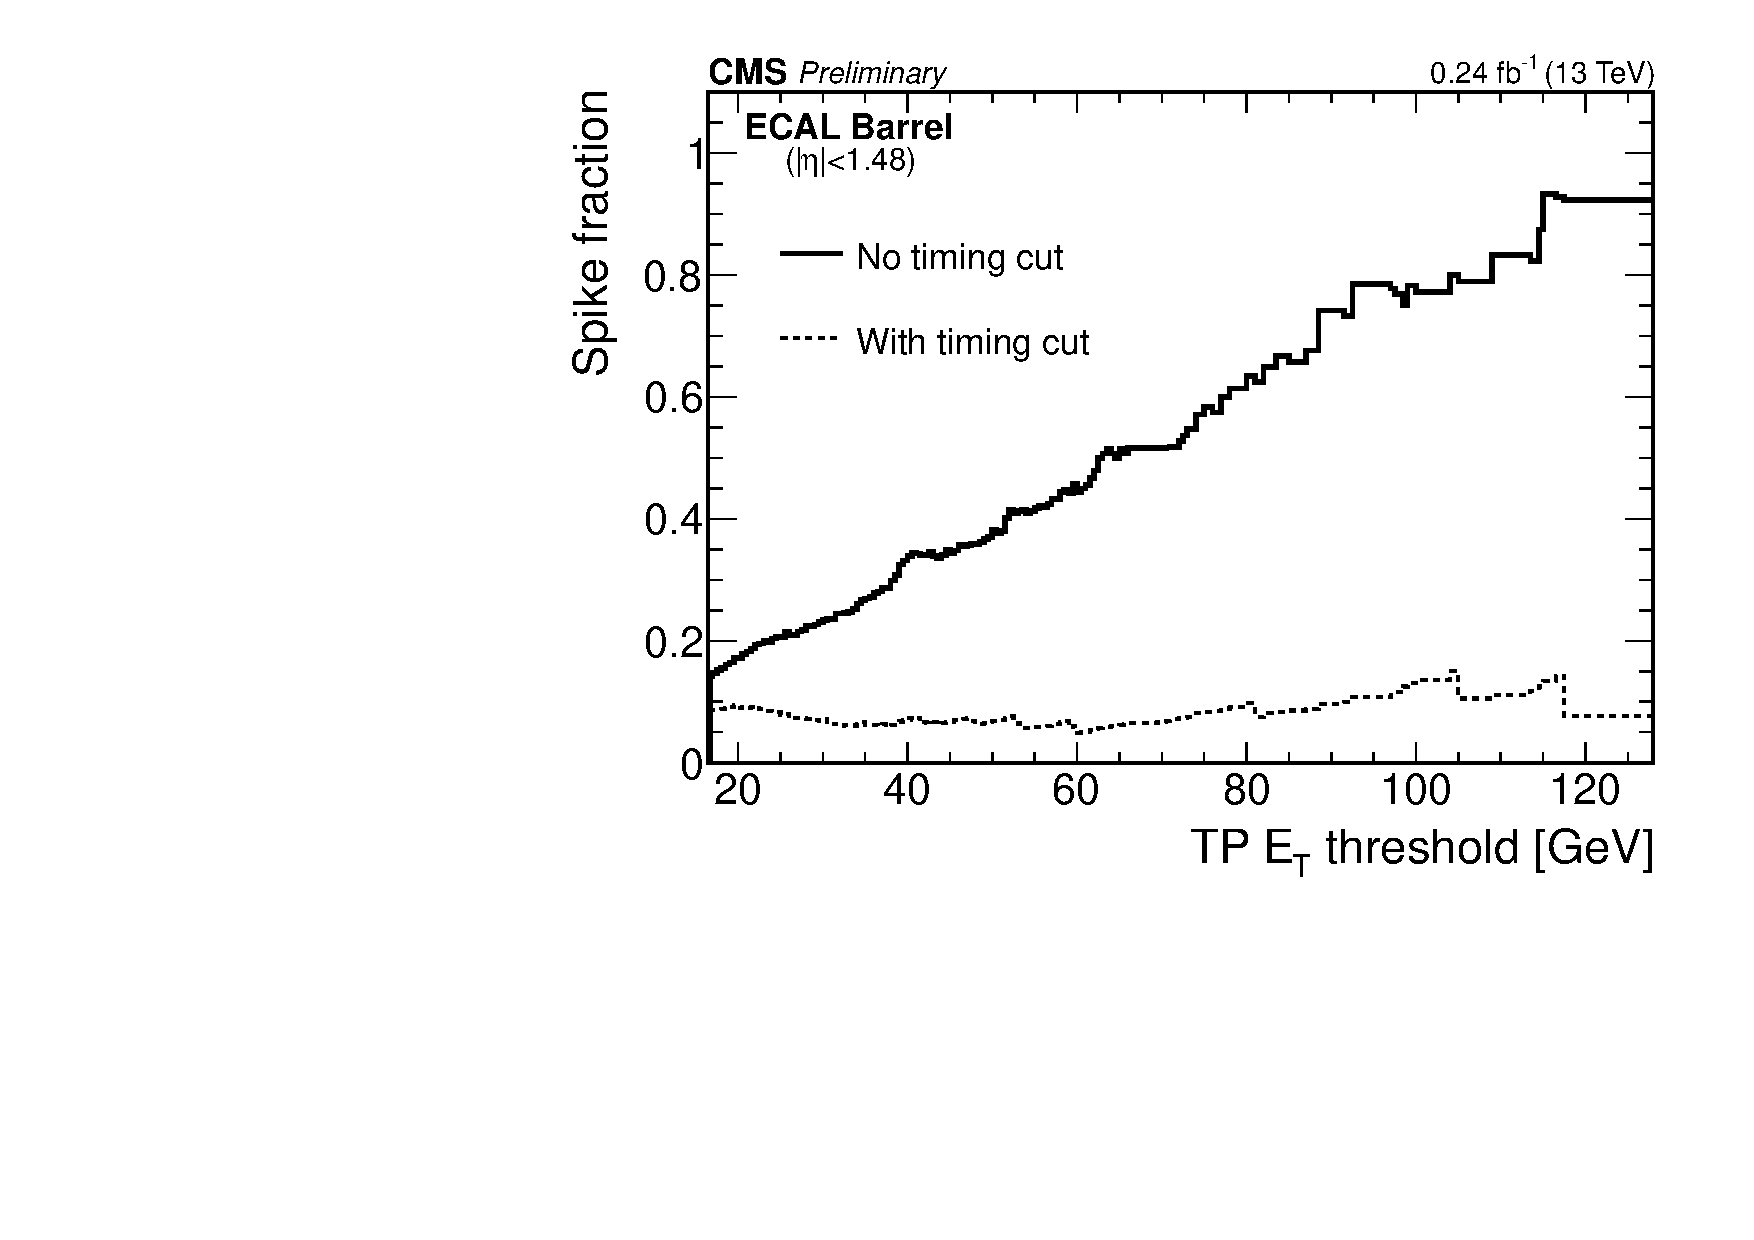
\includegraphics[width=0.49\textwidth]{Images/ECAL/DW/spikecontamination_beforeaftertimingcut.pdf}}%
    \caption{Spike quantities with/without timing cut \href{https://twiki.cern.ch/twiki/bin/view/CMSPublic/EcalDPGResultsCMSDPS2019031}{[EcalDPGResults]},\href{https://cds.cern.ch/record/2690933/files/DP2019_031.pdf}{[CDS]}}%
    \label{fig:TimingCutSpikeReduction}
\end{figure}     

A timing cut like this is not possible in the ECAL FENIX chip; However this study motivated the idea to use two sets of amplitude weights and a comparator in the FENIX chip in order to identify out-of-time signals with double weights. 

\subsection{Optimization}

In the ECAL FENIX chip, it is possible to compute two amplitudes via two sets of weights, and utilize a comparator in the electronics to set a boolean flag if one amplitude output is greater than the other. If an ODD set of weights is optimized to identify out of time signals, it is expected to returns a greater amplitude for out-of-time signals than the Run 2 weights designed for in-time signals. Therefore, the approach is taken to optimize an ODD set of weights for out-of-time signals.

Choosing an odd set of weights for out-of-time signal tagging is a multivariate problem, which must consider a realistic signal energy spectrum, spike energy spectrum, spike timing PDF, and the effects of pileup on signal waveform distortion. Therefore in order to extract ODD weights sets which are optimized to maximize signal efficiency and spike rejection, a numerical optimization was setup in order to derive optimal sets of weights to take the place of the second FIR filter weights. This optimization makes use of simulated signal waveforms using the alpha-beta analytic representation and simulated pileup described in Section \ref{sec:PU_Optimized_Weights}, and the simulation of spike waveforms from a standalone simulation. The optimization is setup as a loss minimization problem which makes use of gradient descent computation and backwards propagation of loss to maximize the amount of spike rejection, while minimizing the amount of signal rejection. This is incorporated in a loss definition, shown in Figure \ref{fig:NumOptLoss}.

\begin{figure}[H]%
    \setcounter{subfigure}{0} % reset subcaption counter to 0 (a) 
    \centering
    \subfloat[Loss function]{
\includegraphics[width=0.31\textwidth]{Images/ECAL/DW/LossFunction.png}}%
    \hfill
    \subfloat[Use of $\delta_{min}$ in loss]{
\includegraphics[width=0.31\textwidth]{Images/ECAL/DW/deltamin_use.png}}%
    \hfill
    \subfloat[Definition of ODD weights loss limit.]{
\includegraphics[width=0.31\textwidth]{Images/ECAL/DW/W2LossLimit.png}}
    \caption{Loss definition used in optimization of ODD set of amplitude weights.}%
    \label{fig:NumOptLoss}
\end{figure}  

One of the input parameters in the optimization is a minimum separation of the two amplitude values computed by the EVEN (default weights) and ODD (out-of-time sensitive) sets of weights, termed $\delta_{min}$. Varying this parameter results in different working points. The different portions of a simulated spike timing PDF which were tagged as out of time by different working points is shown in Figure \ref{fig:DW_StandaloneSimulation_SpikeTimingPDFTagging} \cite{CMS-DP-2022-007, CMS-DP-2022-007_Plots}. 

\begin{figure}[H]
    \centering
    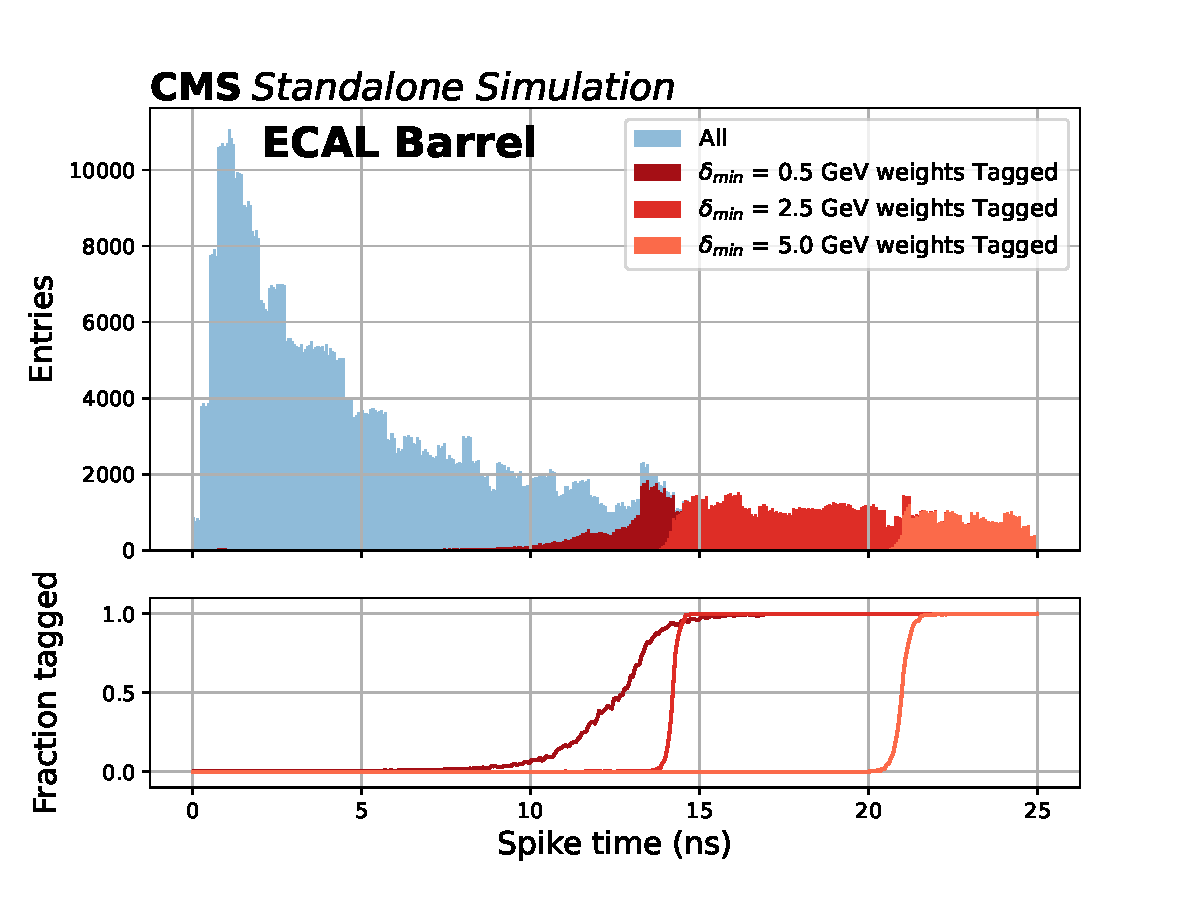
\includegraphics[width=0.8\textwidth]{Images/ECAL/DW/Double_Amplitude_Weights_SpikeTaggingwithOOTWeights_allDeltaMins.pdf}
    \caption{Tagging of out of time spikes in a standalone simulation.}
    \label{fig:DW_StandaloneSimulation_SpikeTimingPDFTagging} 
\end{figure}

In the spike timing PDF, most spikes are relatively in-time with respect to EM signals, while a non-negligible fraction have a late out of time tail. The reason for this is because spike progenitors often spend time propagating in the CMS detector before directly ionizing the EB APDs. It can be seen that increasing the value of the $\delta_{min}$ parameter tags later out of time spikes. This is somewhat expected, as a larger $\delta_{min}$ value will only use spike examples with larger differences in EVEN and ODD amplitudes in its optimization, which is more likely to come from out-of-time shifted spikes. 

While quantifying the expected gain in spike rejection from different $\delta_{min}$ working points, it is also important to check their effect on EM shower-like signals, as shown for a standalone simulation in Figure \ref{fig:SimSignaltaggedvsE}. 

\begin{figure}[H]
    \centering
    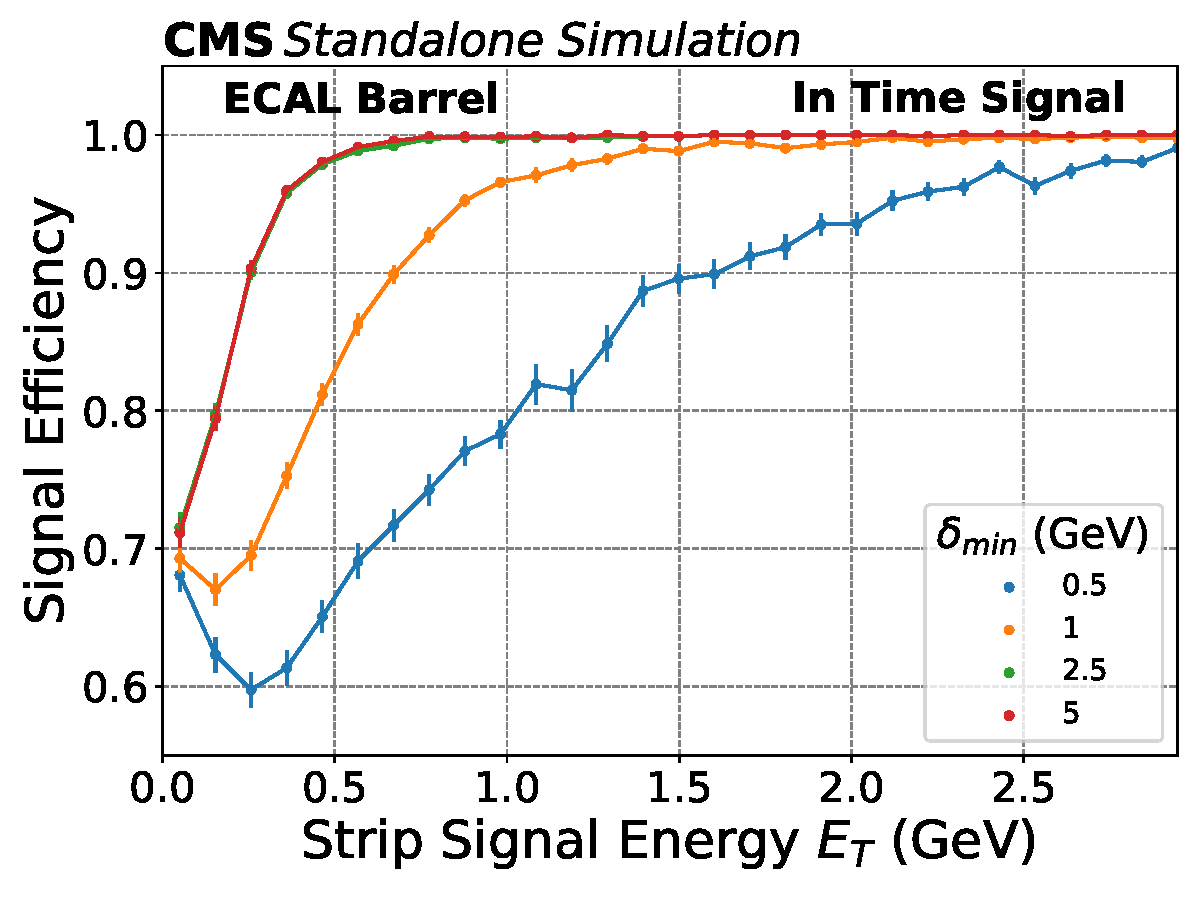
\includegraphics[width=0.8\textwidth]{Images/ECAL/DW/SigEff_vs_SigET.pdf}
    \caption{Signal efficiency vs. signal energy using a standalone simulation and simulation of ECAL double weights algorithm.}
    \label{fig:SimSignaltaggedvsE}
\end{figure}

It is observed that increasing the $\delta_{min}$ parameter value results in higher signal efficiency, as expected for the same reason that a greater spike rejection is observed for greater $\delta_{min}$ values: Only signal and spike waveforms which exhibit larger differences in EVEN and ODD amplitudes are used for weight optimization, leading to weights which are more optimized for very different waveforms and therefore less likely to touch signal waveforms. In order to identify a reasonable trade-off between signal efficiency and spike rejection, the resulting efficiencies are rejections for different $\delta_{min}$ working points is shown in Figure \ref{fig:SpikeRejSigEffTable}, where only signals with $E_{T} \leq 3$ GeV are considered as simulated signals with $E_{T} > $ 3 GeV have an efficiency near 100\%. Additionally, only spikes with a timing greater than 10 ns are considered, as these working points are not effective at tagging in-time spikes.

\begin{figure}
    \centering
        \begin{tabular}{|c|c|c|} \hline 
          $\delta_{min}$ (GeV) & Signal efficiency (\%) & Spike rejection (\%) \\ \hline 
         0.5 & 78.2 & 77.6 \\ \hline  
         2.5 & 95.6 & 62.5 \\ \hline 
         5.0 & 95.7 & 19.2 \\ \hline    
        \end{tabular}
    \caption{Signal efficiency and spike rejection for different $\delta_{min}$ working points.}
    \label{fig:SpikeRejSigEffTable}
\end{figure}

It is shown that moving from the $\delta_{min} = $ 2.5 GeV to 5.0 GeV working point returns a minimal gain in signal efficiency (0.1\%), while a large fraction of spike
rejection is lost (43.3\%). This indicates that the $\delta_{min} = 2.5$ GeV working point provides a good compromise between signal efficiency at low $E_{T}$ and overall spike rejection.

\subsection{Re-emulation of 2018 data} \label{sec:reEmuOf2018Data}

One of the ways to test new features during a long shutdown period when no new data is being taken is be re-emulating previously recorded data. As double weights were an undiscovered feature, they were not present in the CMS ECAL emulator. After verifying the existence of this feature in hardware through tests at CERN building 904 and at the CMS ECAL itself, the now confirmed second amplitude filter was added as a possible configuration in the CMS emulator \cite{CMSSW_DW}.

After including this implementation in the centrally used CMS software, 2018 CMS data was re-emulated using ECAL double weights in order to see how this would have affected data-taking. Double weights were run in "Killing mode", meaning that if an ECAL strip has a higher ODD amplitude than EVEN amplitude, its energy is set to zero. The idea behind this is to zero spikes which are often out-of-time, while trying to minimize the zeroing of signals which are in-time. 

In order to categorize ECAL TPs in data as signal-like or spike-like, an offline ``Severity" assignment is used. Each EB TT (Trigger tower) is composed of 25 ECAL crystals. An offline energy computation is performed for each crystal in highly energetic regions of events with an L1A, called a reconstructed hit or ``rec hit". In addition, a timing value is computed for each reconstructed hit, and a ``severity" level is assigned. A severity level of 0 corresponds to a reconstructed hit which does not appear problematic in the data. A severity level of 3 means a reconstructed hit is identified as out-of-time based on its reconstructed timing value, and a severity level of 4 means a reconstructed hit satisfies at least one of the following: Identified as out-of-time based on its reconstructed time value, fails a topological cut, known as a ``swiss-cross" cut. Because spikes come from isolated APD hits, rather than from a spread-out EM shower with energy spread over a group of ECAL crystals, spikes usually have their energy fully deposited in one crystal and are identified using a swiss cross variable, shown in Figure \ref{fig:SwissCross}. Thus, severity zero (four) reconstructed hits typically correspond to signal-like (spike-like) hits shown in its respective region of reconstructed time vs. swiss-cross score in Figure \ref{fig:TimeVsSwissCross} \cite{CMS-DP-2012-008, CMS-DP-2012-008_Plots}. 

\begin{figure}[H]%
    \setcounter{subfigure}{0}
    \centering
    \subfloat[Swiss cross definition, illustrated by the energy hits in a 3x3 ECAL crystal portion. E1 = energy of the central crystal, E4 = sum of the energies of the central crystal's four surrounding neighbors.  \label{fig:SwissCross}]{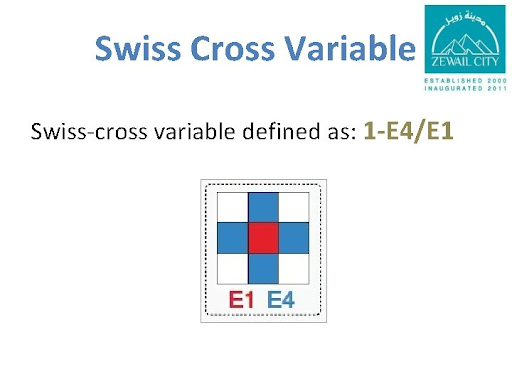
\includegraphics[width=.475\textwidth]{Images/ECAL/DW/SwissCross.png}}%
    \hfill
    \subfloat[Reconstructed time vs. swiss cross score \label{fig:TimeVsSwissCross}]{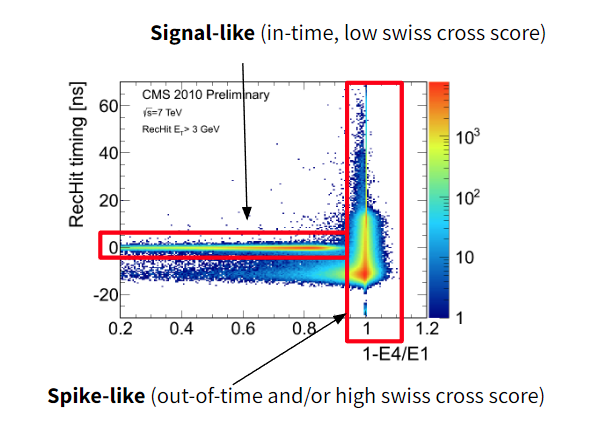
\includegraphics[width=.475\textwidth]{Images/ECAL/DW/timeVsSwissCross.png}}%
    \caption{Swiss cross definition, and reconstructed hit timing vs. swiss cross score from a 2010 CMS data sample.}%
\end{figure}

In order to assign a severity level and reconstructed time to an EB TP, the severity level and reconstructed time of the highest energy reconstructed hit in a given TP is assigned to that TP, as shown in Figure \ref{fig:RecHitTPMatching}. In this example TP with reconstructed crystal energies in arbitrary units, the highest energy reconstructed hit is in Strip 3, crystal 0 as its value is 201, and thus this TP is assigned the timing and severity of this crystal. 

\begin{figure}[H]
    \centering
    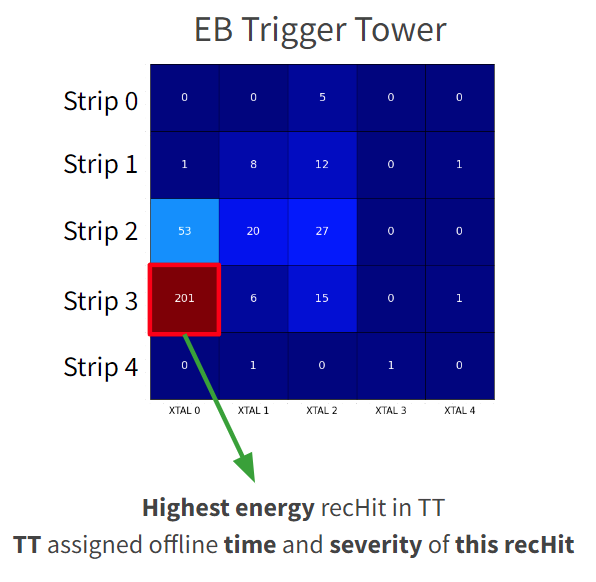
\includegraphics[width=0.8\textwidth]{Images/ECAL/DW/TPRecHitMatching.png}
    \caption{Reconstructed hit matching to TP. Crystal energy units are arbitrary.}
    \label{fig:RecHitTPMatching}
\end{figure}

In the re-emulation of 2018 CMS data, the resulting 1 - emu/real distributions, where emulated energy includes double weights in killing mode, and real energy corresponds to the energy of the TP from data with no double weights applied, are shown in Figure \ref{fig:2018Reemulation_KillingMode} for signals (TPs assigned to severity 0 reconstructed hits) which are in time (matched reconstructed crystal hit time $|t| < 3$ns), and spikes (TPs assigned to severity 4 reconstructed hits) which are out-of-time (matched reconstructed crystal hit time $t > 10$ns). 

\begin{figure}[H]%
    \setcounter{subfigure}{0}
    \centering
    \subfloat[2018 CMS data re-emulation, in time severity zero energies in killing mode \label{fig:DW_2018Reemulation_InTimeSevZeroKillingMode}]{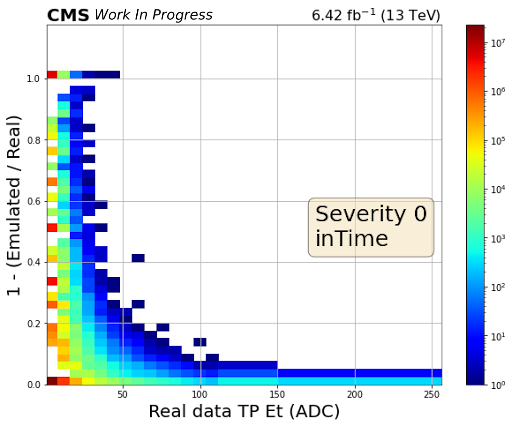
\includegraphics[width=.475\textwidth]{Images/ECAL/DW/DW_2018_Reemulation_InTimeSevZeroEnergies.png}}%
    \hfill
    \subfloat[2018 CMS data re-emulation, very late severity four energies in killing mode \label{fig:DW_2018Reemulation_VeryLateSevFourKillingMode}]{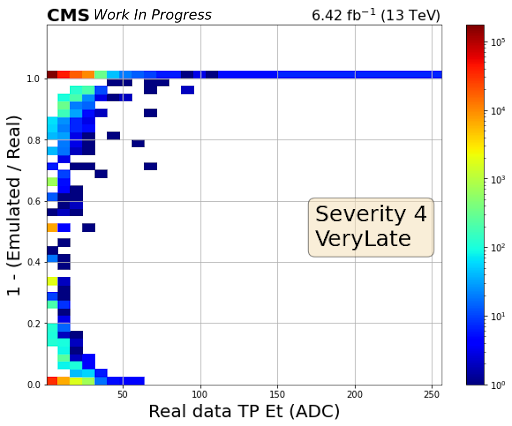
\includegraphics[width=.475\textwidth]{Images/ECAL/DW/DW_2018_Reemulation_VeryLateSevFourEnergy.png}}%
    \caption{2018 Data reemulation with double weights in killing mode. \label{fig:2018Reemulation_KillingMode}}%
\end{figure}

This shows that relatively high energy spikes, greater than about 50 ADC (25 GeV), are being mostly zeroed, shown by the fact that the 1 - emulated / real is close to one, meaning the emulated (TP energy with double weights in killing mode) energy is nearly zeroed. There is also a non-negligible amount of zeroing being applied to in-time signals, as the per y-slice distributions show some entries greater than 0. 

To check the timings of TPs which have some energy subtracted by double weights in the full timing range, not just restricted to in time and very later, we can observe the data TP vs. its offline assigned time for all TPs shown in Figures \ref{fig:All_Sev_zero} and \ref{fig:All_Sev_four}, and for TPs in which at least 90\% of energy is removed by double weights in killing mode in figures \ref{fig:MostlyZeroed_Sev_zero} and \ref{fig:MostlyZeroed_Sev_four}. For both severity categories, a line is drawn at 32 ADC, equivalent to 16 GeV for ECAL TPs, as this is the spike killing threshold as defined in Section \ref{sec:spikes}. 

\begin{figure}[H]%
    \setcounter{subfigure}{0}
    \centering
    \subfloat[All severity zero TPs \label{fig:All_Sev_zero}]{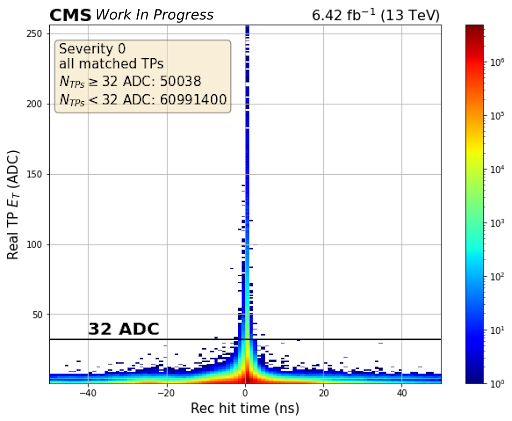
\includegraphics[width=.475\textwidth]{Images/ECAL/DW/DW_2018_Reemulation_AllSevZeroTPs.png}}%
    \hfill
    \subfloat[Severity zero TPs mostly zeroed \label{fig:MostlyZeroed_Sev_zero}]{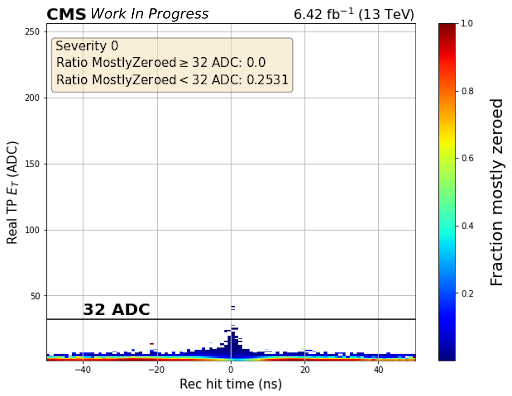
\includegraphics[width=.475\textwidth]{Images/ECAL/DW/DW_2018_Reemulation_SevZeroTPsMostlyZeroed.png}}%
    \caption{2018 Data reemulation - severity 0 TPs \label{fig:A}}%
\end{figure}

\begin{figure}[H]%
    \setcounter{subfigure}{0}
    \centering
    \subfloat[All severity four TPs \label{fig:All_Sev_four}]{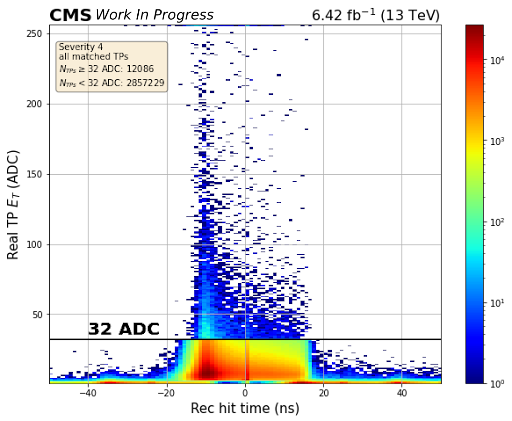
\includegraphics[width=.475\textwidth]{Images/ECAL/DW/DW_2018_Reemulation_AllSevFourTPs.png}}%
    \hfill
    \subfloat[Severity four TPs mostly zeroed \label{fig:MostlyZeroed_Sev_four}]{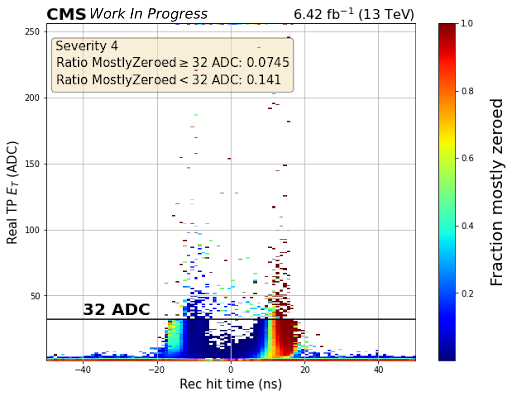
\includegraphics[width=.475\textwidth]{Images/ECAL/DW/DW_2018_Reemulation_SevFourTPsMostlyZeroed.png}}%
    \caption{2018 Data reemulation - severity 4 TPs \label{fig:A}}%
\end{figure}

In the distributions containing all TPs, most signals are in-time as expected. It is also observed that a large portion of spikes are out of time, as expected. It is observed that many spikes have a negative timing around -12.5ns, which is due to a bias in the ECAL offline energy reconstruction, which is optimized for signal waveforms which are slightly different from spike waveforms. Spike waveforms with a negative reconstructed time are generally expected to really be in time. Additionally, the effect of the spike killer is visible for severity four TPs, as there is a sharp drop-off in the number of TP entries above the spike killer threshold of 32 ADC (16 GeV). 

The distributions of TPs which have at least 90\% of their energy subtracted by double weights in killing mode show that most signal-like TPs which are mostly zeroed are very low energy and out of time, which are likely coming from noise, and it can be seen that there is a non-zero chance of some in-time signal energy subtraction. For spike TPs, it is seen that the majority of TPs which have their energy mostly subtracted are positively out of time, as expected with double weights based on the standalone simulation shown in Figure \ref{fig:DW_StandaloneSimulation_SpikeTimingPDFTagging}. The spike contamination of ECAL TPs, with and without double weights activated in killing mode, is shown in Figure \ref{fig:DW_2018Reemulation_SpikeContamination}. 

\begin{figure}[H]
    \centering
    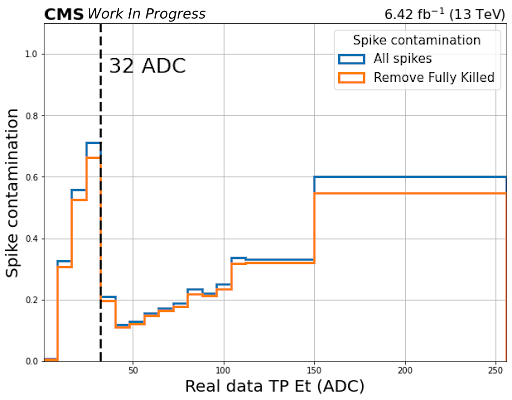
\includegraphics[width=0.8\textwidth]{Images/ECAL/DW/SpikeContamination_DoubleWeights.png}
    \caption{2018 CMS data re-emulation, expected improvement in spike contamination, including below the spike killer threshold.}
    \label{fig:DW_2018Reemulation_SpikeContamination}
\end{figure}

This shows that with ECAL double weights, there is some potential to lower the spike contamination rate, including in the high energy regime. This is also true for spikes with energy less than 32 ADC (16 GeV), the existing Level-1 spike killer threshold. 

While we see potential for a decrease in spike contamination, this re-emulation of 2018 CMS data also showed we may expect to have the unwanted removal of some signal energy at low TP energies with this double weights working point. In order to further study this, another re-emulation was performed with a full-readout ECAL run. The reason a full-readout run was included in this study is because in full-readout, information from all ECAL crystals is saved. In non full-readout runs, there is a selective readout procedure in which low interest regions are not readout. It is desirable to re-emulate full readout runs when comparing low energy TP energies between data and re-emulation, to ensure that all ECAL information is available for emulation in order to have a proper comparison to data. This re-emulation was performed with two double weights working points: $\delta_{min}$ = 0.5 and 2.5 GeV, running with double weights in killing mode. The resulting average energy fractions subtracted from in time signals and out-of-time spikes when re-emulating with these two working points are shown in Figure \ref{fig:2018Reemulation_FR_KillingMode_deltamincompare}. 

\begin{figure}[H]%
    \setcounter{subfigure}{0}
    \centering
    \subfloat[In time severity zero TPs \label{fig:2018Reemulation_FR_KillingMode_deltamincompare_InTimeSignals}]{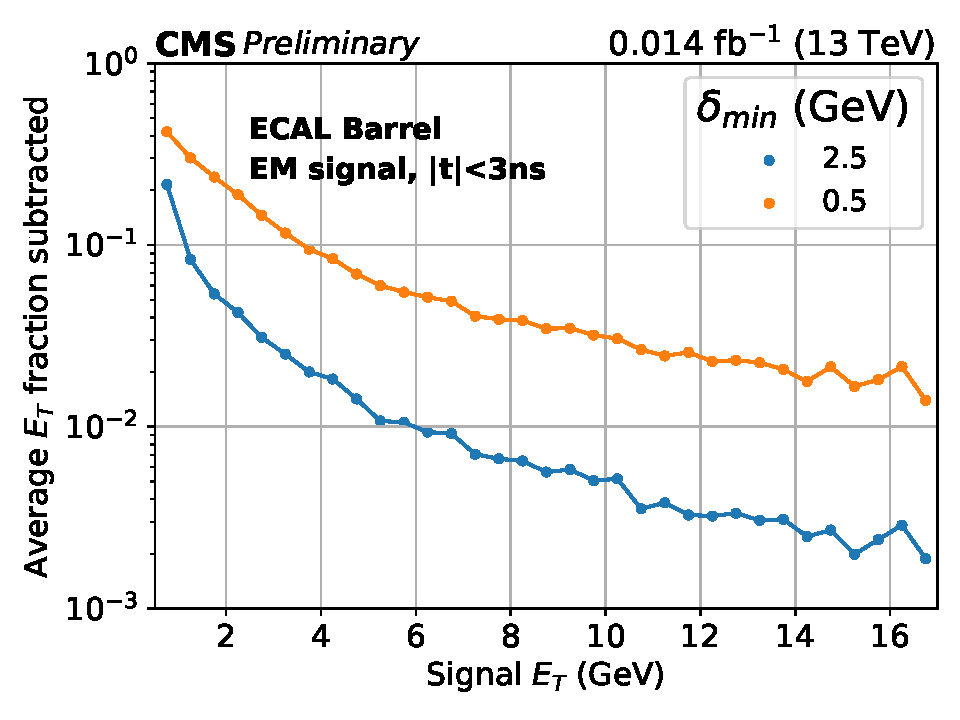
\includegraphics[width=.475\textwidth]{Images/ECAL/DW/Sev_zero_inTime_Average_oneMinusEmuOverRealvstwrADCCourseBinningZoomed_log.pdf}}%
    \hfill
    \subfloat[Very late severity four TPs \label{fig:2018Reemulation_FR_KillingMode_deltamincompare_VeryLateSpikes}]{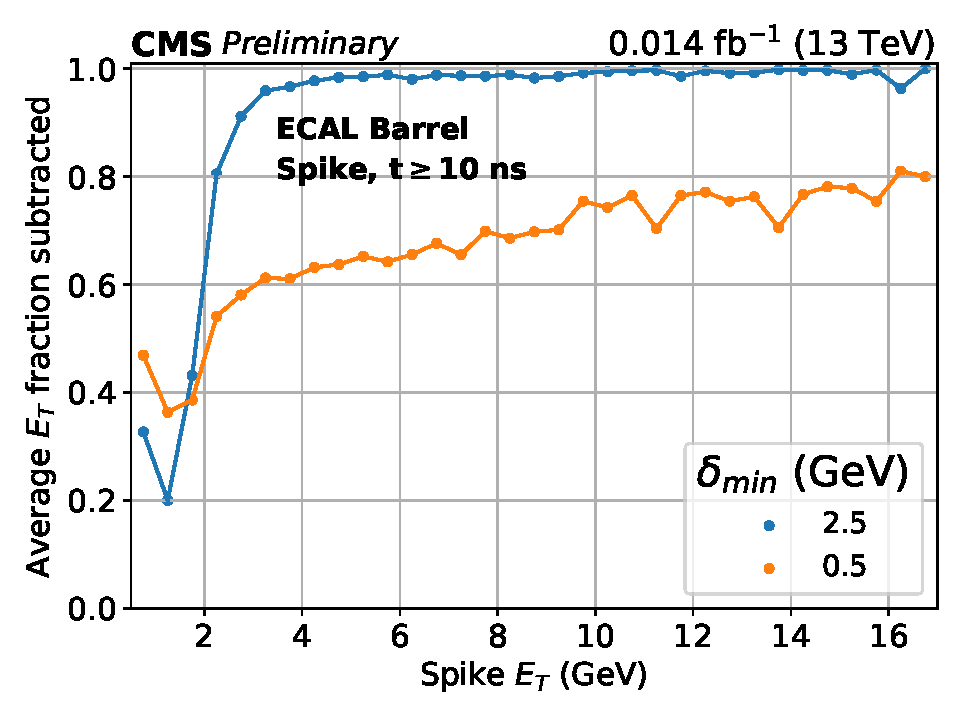
\includegraphics[width=.475\textwidth]{Images/ECAL/DW/Sev_four_VeryLate_Average_oneMinusEmuOverRealvstwrADCCourseBinningZoomed_linear.pdf}}%
    \caption{2018 Data reemulation, Full Readout run, with DW in killing mode. \label{fig:2018Reemulation_FR_KillingMode_deltamincompare}}%
\end{figure}

Firstly, this re-emulation with the $\delta_{min}$ = 0.5 GeV point shows similar trends observed in the previous study: Namely that low energy signals have a non-zero probability of having energy subtracted which decreases as the TP energy increases, and that out of time spikes have a large percentage of energy subtracted, which increases as spike energy increases. Secondly, both trends exhibit more desirable behavior with the $\delta_{min}$ = 2.5 GeV working point: The amount of signal energy subtraction is decreased, and the amount of spike energy subtraction is increased. These same trends were observed in the standalone simulation results in Figure \ref{fig:DW_StandaloneSimulation_SpikeTimingPDFTagging} for simulated spikes and Figure \ref{fig:SimSignaltaggedvsE} for simulated signals.

\subsection{Commissioning for LHC Run 3} \label{sec:ECALTrigger_Run3}

During the commissioning of CMS and LHC for Run 3, the accelerator complex provided beam splashes to the experiments, in which an LHC collimator upstream from CMS is closed, resulting in a proton bunch interaction and production of a shower of particles, chiefly muons, which traverse the entire CMS detector. An event display from a 2021 LHC beam splash is shown in Figure \ref{fig:2021PilotBeam_BeamSplash}, where red represents ECAL activity and blue represents HCAL activity. 

\begin{figure}[H]
    \centering
    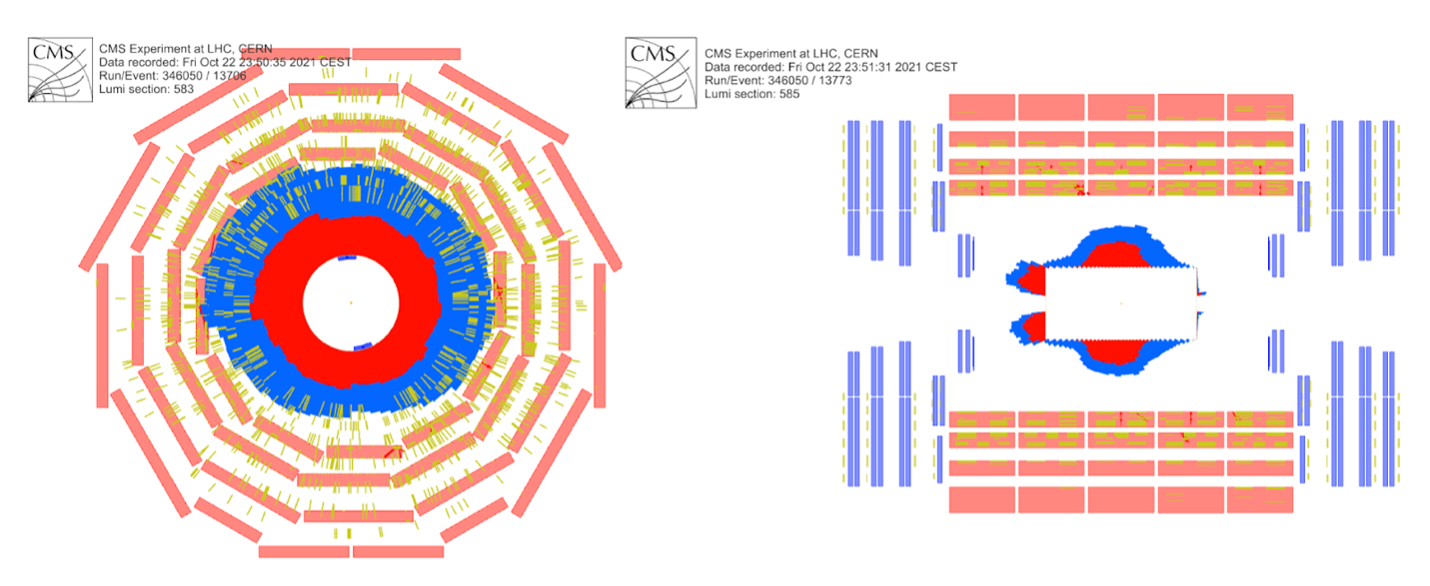
\includegraphics[width=\textwidth]{Images/ECAL/DW/BeamSplash.png}
    \caption{2021 LHC pilot beam: Beam splash}
    \label{fig:2021PilotBeam_BeamSplash}
\end{figure}

During beam splashes, a broad range of ECAL reconstructed hit timings are returned. This is because a shower of particles arrives at the detector from one direction, where CMS is configured to trigger the event from ECAL activity in the central region around $\eta$ = 0. This defines in-time hits in the detector, akin to the time of a proton-proton bunch collision, and because the shower of particles continues to interact with the rest of ECAL as time passes, all of these hits will be recorded as positively out-of-time. Additionally, all of the hits from the shower of particles which strikes ECAL before the event is triggered will be negatively out-of-time with respect to $\eta$ = 0.  

As this means a large range of timings for offline ECAL crystal reconstructed hits is expected which can be matched to ECAL TPs in the same fashion performed in \ref{sec:reEmuOf2018Data}, the ECAL operations team used the opportunity to run with double weights in tagging mode, in which no energy is subtracted but a flag is set if a TP is marked as out-of-time by the double weights mechanism. The resulting ECAL TP timings, and the TPs which were tagged are shown in Figure \ref{fig:2021_BeamSplash_DWTagging}. 

\begin{figure}[H]%
    \setcounter{subfigure}{0}
    \centering
    \subfloat[TP timing distribution]{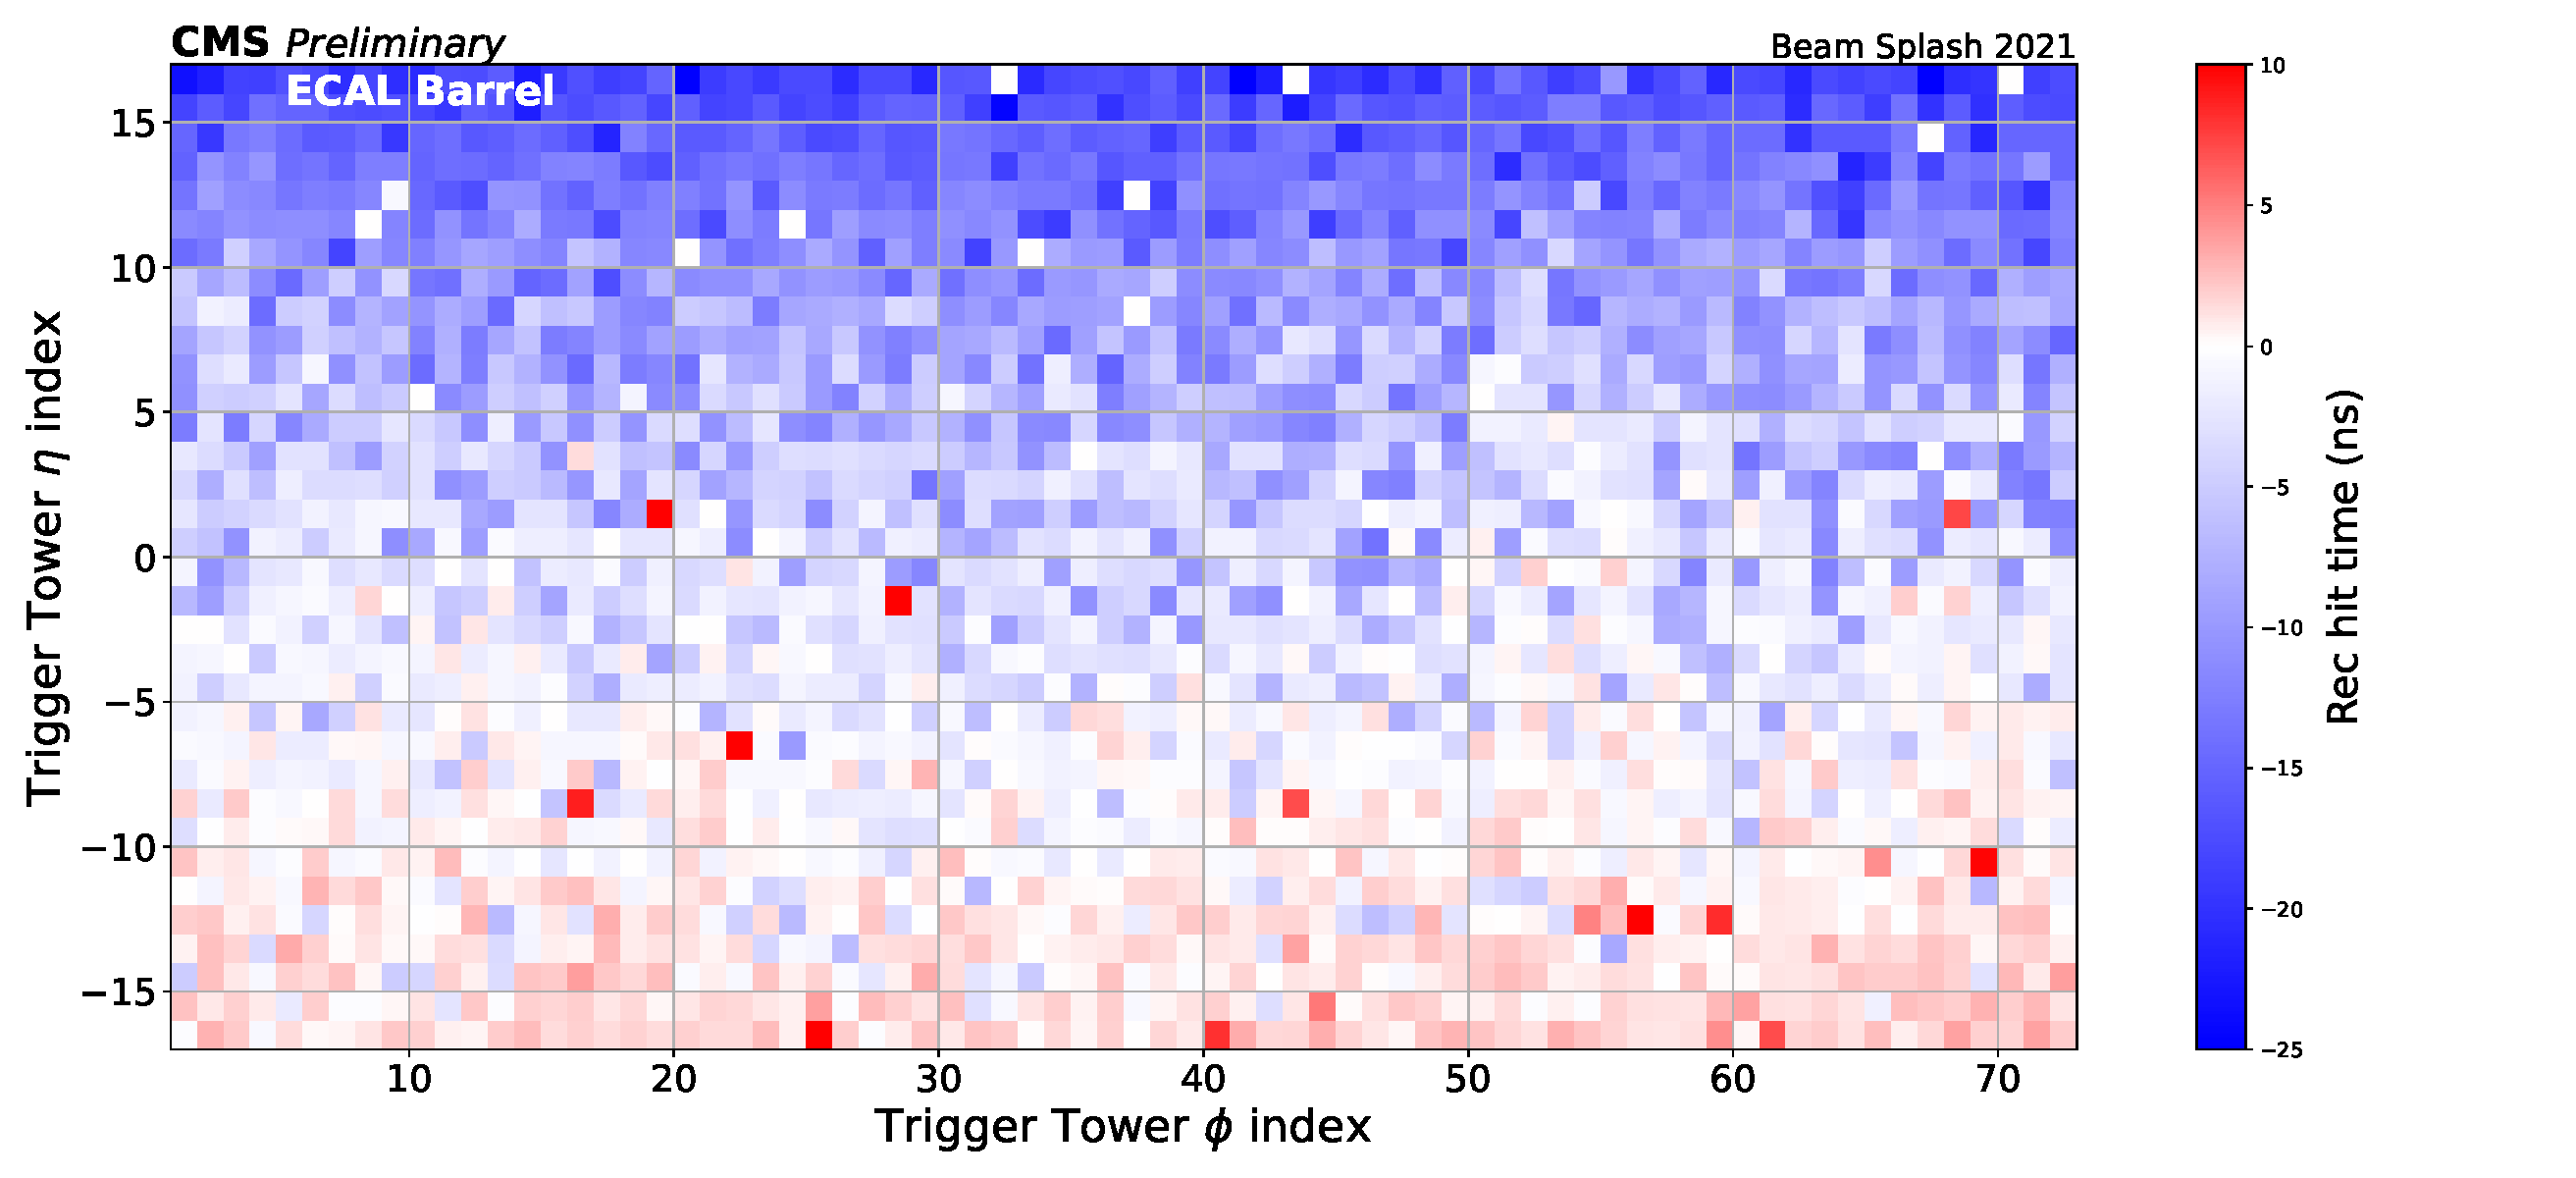
\includegraphics[width=.475\textwidth]{Images/ECAL/DW/BeamSplash2021_time.pdf}}%
    %\hfill
    \subfloat[TPs tagged as out of time]{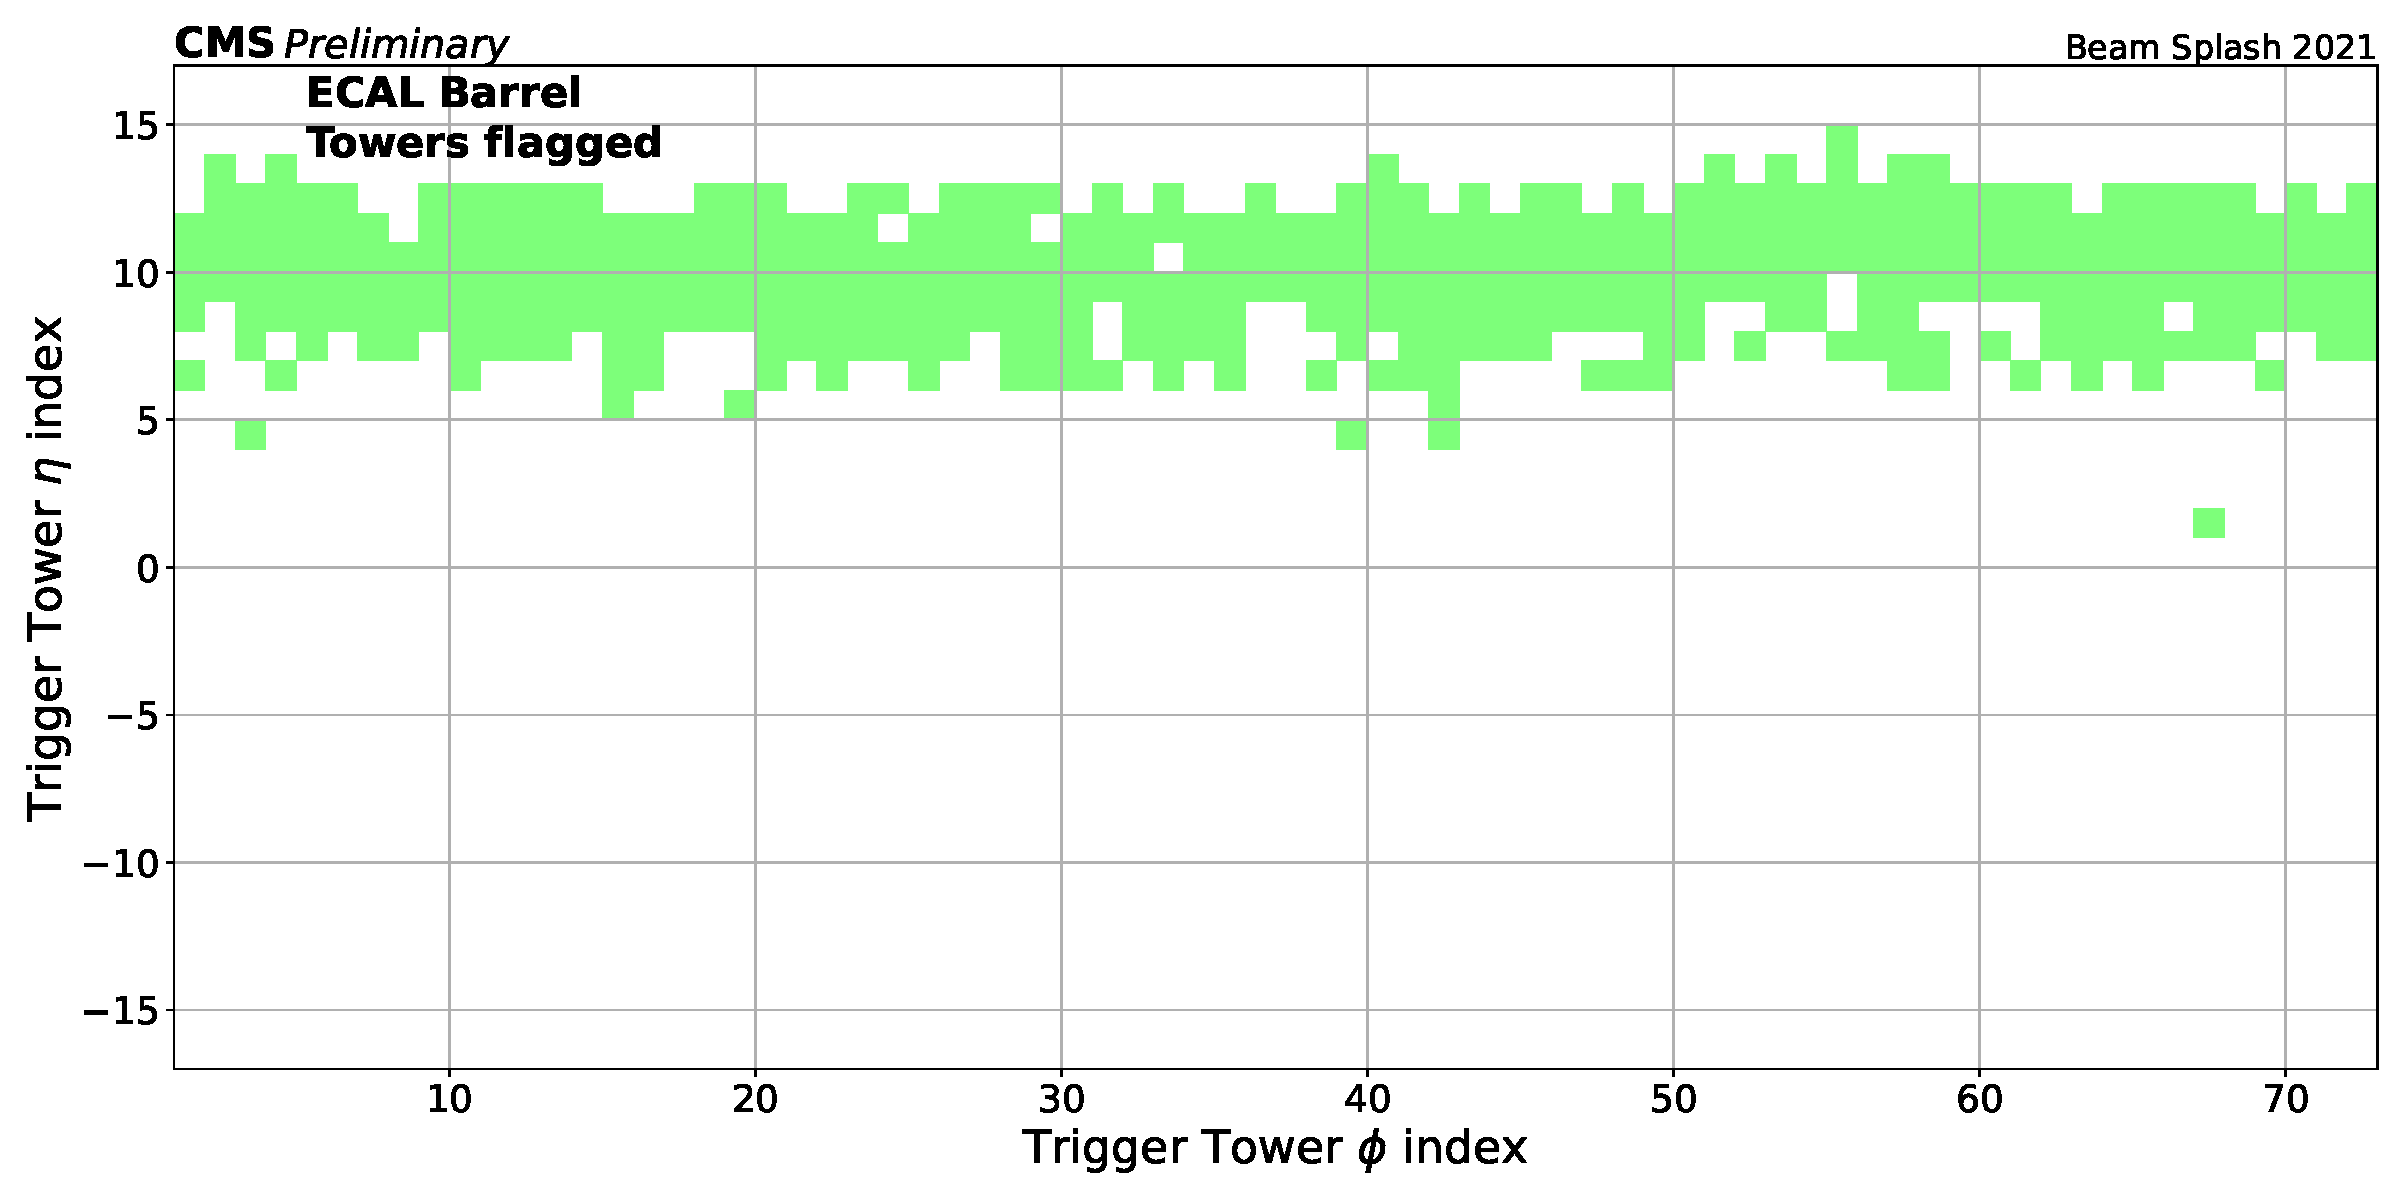
\includegraphics[width=.475\textwidth]{Images/ECAL/DW/BeamSplash2021_FineGrainBit.pdf}}%
    \caption{TP timing distribution, and TPs which are tagged as out-of-time by the double weights mechanism, from a 2021 CMS beam splash. \label{fig:2021_BeamSplash_DWTagging}}%
\end{figure}  

It is observed that the TP timings, obtained by assigning the timing of the highest energy reconstructed hit in the TT, range from about -25ns to 10ns. The TPs which are tagged by the double weights mechanism as out-of-time have timings in the largely negative region of about -10 ns to -15 ns, with no tagging of in-time signals. This marked the first instance of out-of-time tagging at the ECAL TP level, and proved the functionality of the double weights mechanism for tagging out-of-time signals in data.

In addition, during the 2021 and 2022 LHC commissioning periods, CMS received low intensity 900 GeV center-of-mass energy collisions. During a 2 hour period, ECAL took data from these collisions in full readout mode running with double weights in tagging mode, in a 2021 run with the $\delta_{min}$ = 0.5 GeV working point, and in a 2022 run with the $\delta_{min}$ = 2.5 GeV working point. For the 2021 run, the data TP energies vs. offline matched times, and the fraction of TPs tagged over the total are shown in Figure \ref{fig:2021_Pilotbeam_TPsallAndTagged_sev0} for severity zero matched signal-like TPs, and Figure \ref{fig:2021_Pilotbeam_TPsallAndTagged_sev4} for severity 4 matched spike-like TPs. 

\begin{figure}[H]%
    \setcounter{subfigure}{0}
    \centering
    \subfloat[All severity 0 signal TPs: Data energy vs. time]{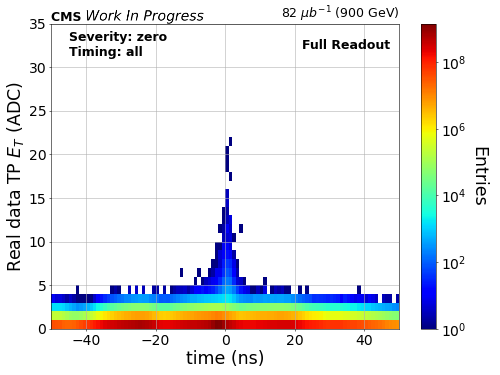
\includegraphics[width=.475\textwidth]{Images/ECAL/DW/2021PilotBeam_Energyvstime_sev0.png}}%
    \hfill
    \subfloat[Signal TPs tagged by double weights with $\delta_{min}$ = 0.5 GeV working point]{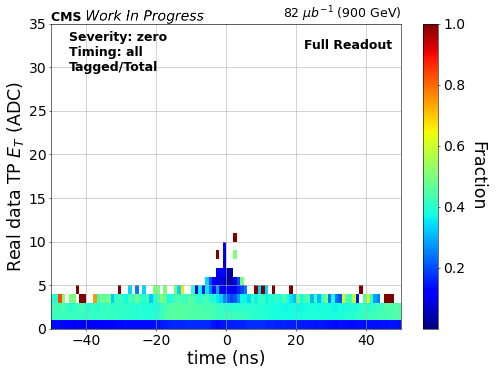
\includegraphics[width=.475\textwidth]{Images/ECAL/DW/2021PilotBeam_Energyvstime_sev0_tagged.png}}%
    \caption{2021 LHC pilot beam severity 0 signal TPs, all and tagged \label{fig:2021_Pilotbeam_TPsallAndTagged_sev0}}%
\end{figure}  

\begin{figure}[H]%
    \setcounter{subfigure}{0}
    \centering
    \subfloat[All severity 4 spike TPs: Data energy vs. time]{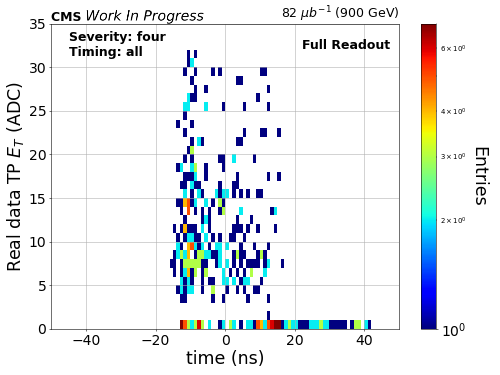
\includegraphics[width=.475\textwidth]{Images/ECAL/DW/2021PilotBeam_Energyvstime_sev4.png}}%
    \hfill
    \subfloat[Spike TPs tagged by double weights with $\delta_{min}$ = 0.5 GeV working point]{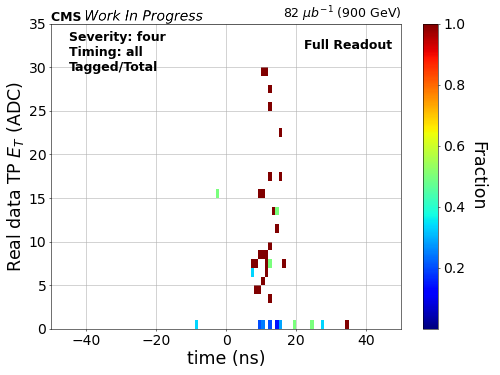
\includegraphics[width=.475\textwidth]{Images/ECAL/DW/2021PilotBeam_Energyvstime_sev4_tagged.png}}%
    \caption{2021 LHC pilot beam severity 4 spike TPs, all and tagged \label{fig:2021_Pilotbeam_TPsallAndTagged_sev4}}%
\end{figure}  

From these distributions, similar behavior is observed compared to that from the 2018 non full-readout and full-readout data re-emulation: Double weights are able to tag TPs which are positively out-of-time, as well as some spikes which are negatively out of time. For signals, there is a non-negligible amount of tagging seen for in-time signals. As the $\delta_{min}$ = 2.5 GeV working point was seen in 2018 re-emulation to have decreased signal tagging and increased spike tagging, the 2022 run with this working point is compared to the 2021 run as shown in Figure \ref{fig:2021_2022_900GeVCollisions_inTimeSignalTagging} for in-time severity 0 matched TPs, and Figure \ref{fig:2021_2022_900GeVCollisions_VeryLateSpikeTagging} for very late severity 4 matched TPs.

\begin{figure}[H]%
    \setcounter{subfigure}{0}
    \centering
    \subfloat[Linear y-scale]{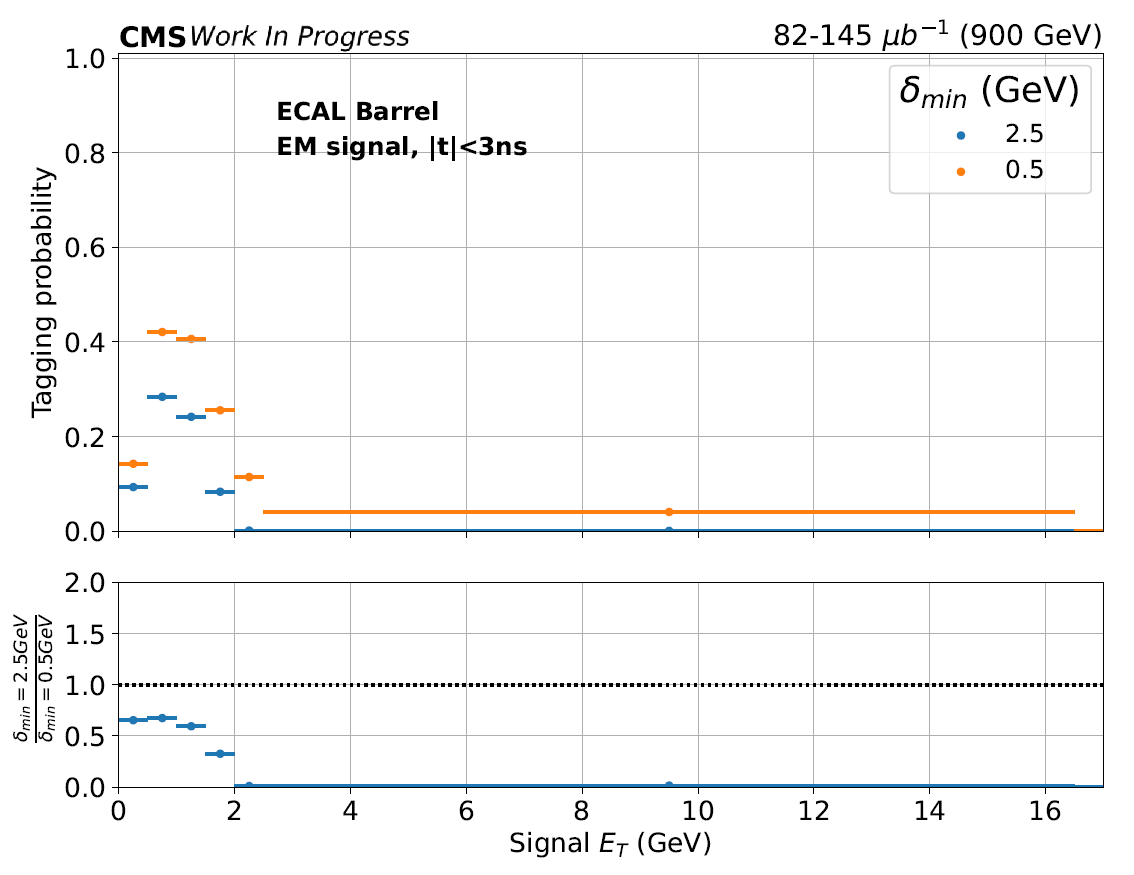
\includegraphics[width=.475\textwidth]{Images/ECAL/DW/Sev_zero_inTime_Average_EnergyVsTimeOccupancy_linear.png}}%
    \hfill
    \subfloat[Logarithmic y-scale]{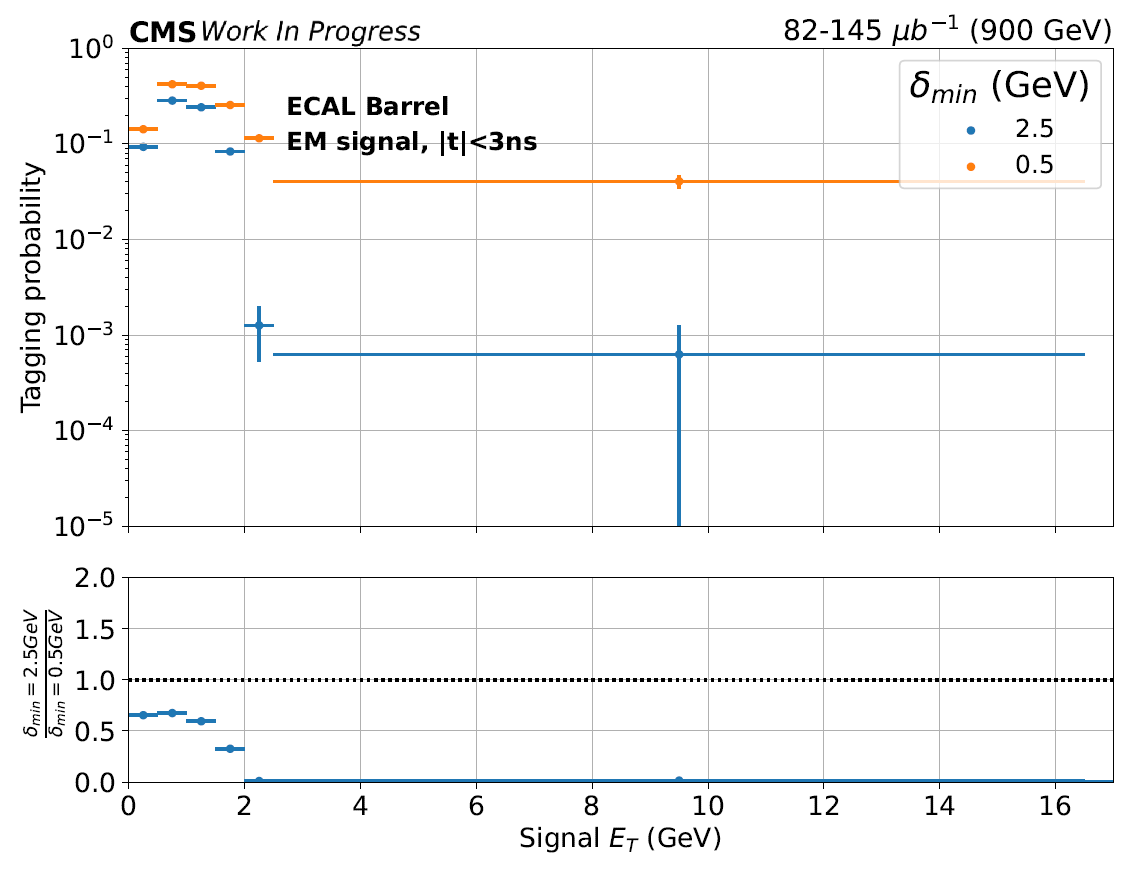
\includegraphics[width=.475\textwidth]{Images/ECAL/DW/Sev_zero_inTime_Average_EnergyVsTimeOccupancy_log.png}}%
    \caption{Tagging probability of in-time signal TPs as a function of TP transverse energy, with two double weights working points, shown in linear and logarithmic y-scale. \label{fig:2021_2022_900GeVCollisions_inTimeSignalTagging}}%
\end{figure}  

\begin{figure}[H]
    \centering
    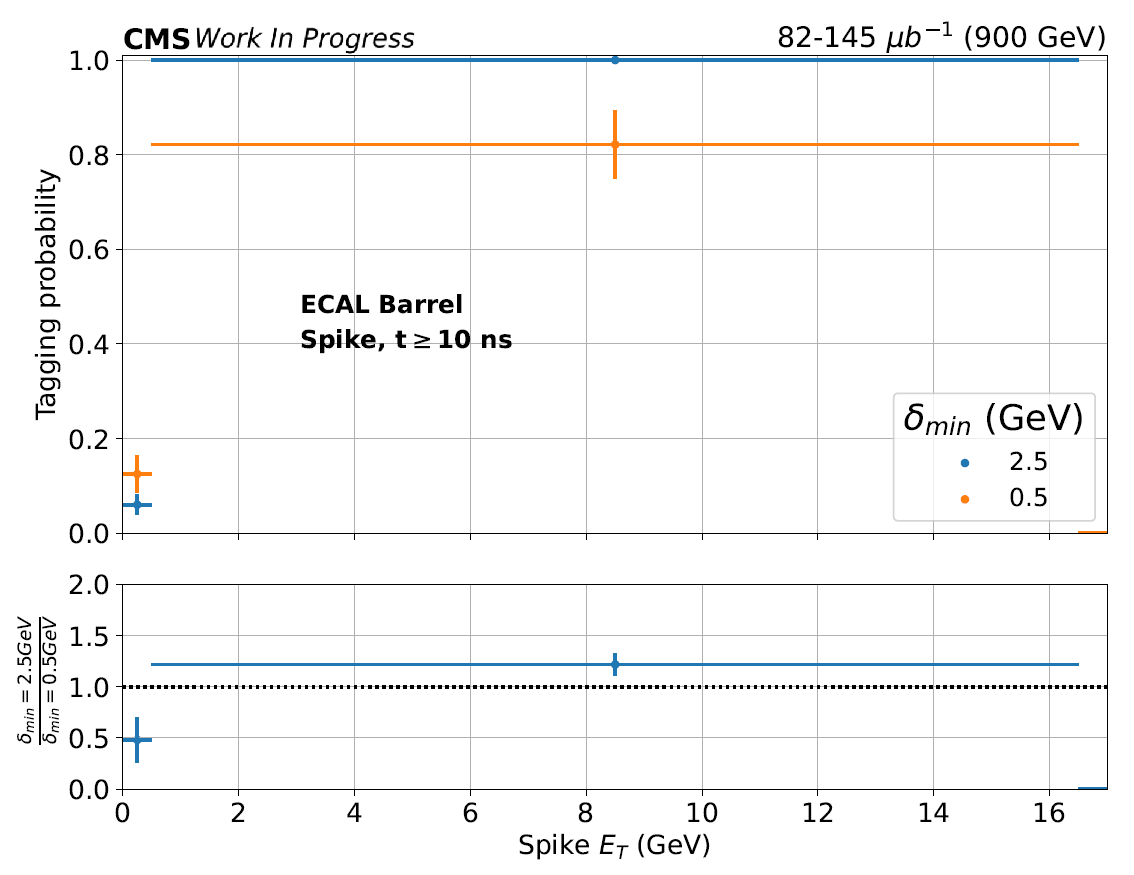
\includegraphics[width=0.9\textwidth]{Images/ECAL/DW/Sev_four_VeryLate_Average_EnergyVsTimeOccupancy_linear.png}
    \caption{Tagging probability of in-time signal TPs as a function of TP transverse energy, with two double weights working points.}
    \label{fig:2021_2022_900GeVCollisions_VeryLateSpikeTagging}
\end{figure}

This comparison returns similar behavior compared to the 2018 full readout re-emualtion shown in Figure \ref{fig:2018Reemulation_FR_KillingMode_deltamincompare}, as the $\delta_{min}$ = 2.5 GeV working point has less in time signal tagging which decreases as energy increases, and more late spike tagging which increases as energy increases.

In order to ensure that the emulator is properly simulating the ECAL double weights tagging mechanism as observed in data, a comparison of the tagging by data and the emulator was investigated for these two low energy runs, shown in Figure \ref{fig:SevZeroDataEmulatorTagging} for in-time severity 0 matched TPs, and Figure \ref{fig:SevFourDataEmulatorTagging} for very late severity 4 matched TPs.

\begin{figure}[H]%
    \setcounter{subfigure}{0}
    \centering
    \subfloat[2021 collisions, $\delta_{min}$ = 0.5 GeV working point ]{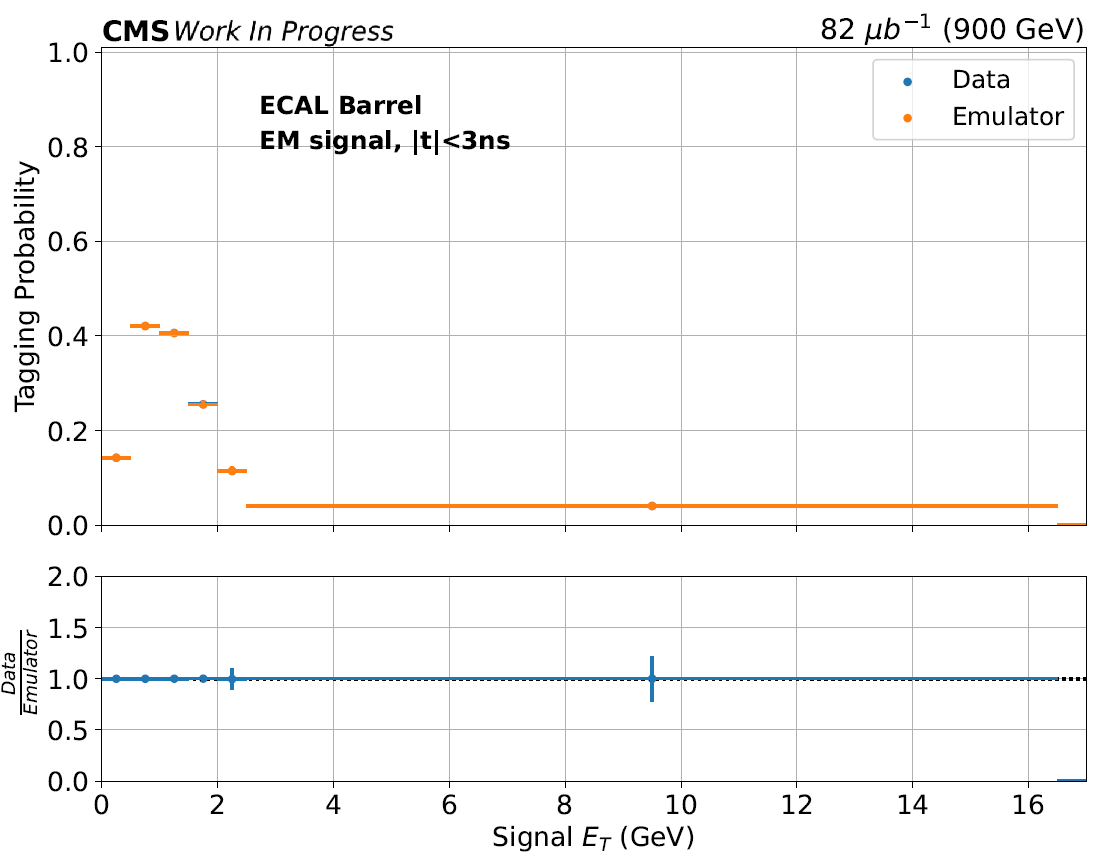
\includegraphics[width=.475\textwidth]{Images/ECAL/DW/2021Collisions_Sev_zero_inTime_DataOverEmulatorTaggingProbability_linear.png}}%
    \hfill
    \subfloat[2022 collisions, $\delta_{min}$ = 2.5 GeV working point]{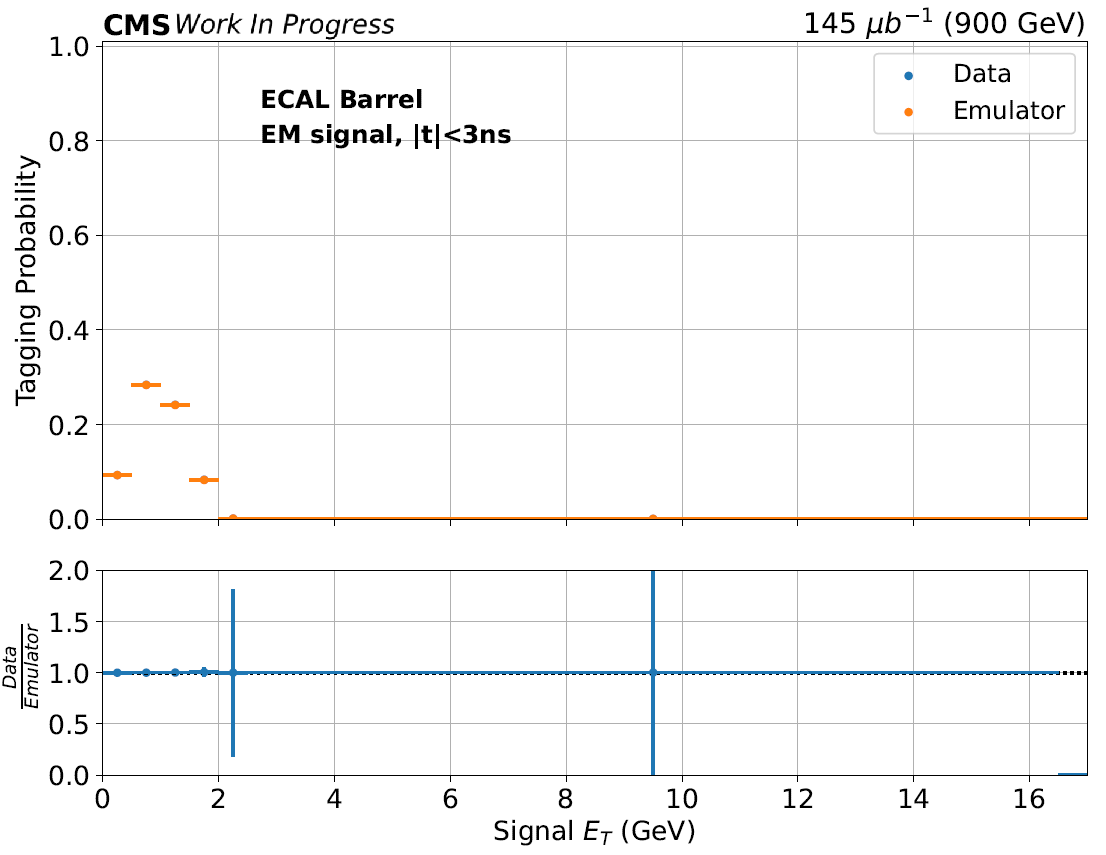
\includegraphics[width=.475\textwidth]{Images/ECAL/DW/2022Collisions_Sev_zero_inTime_DataOverEmulatorTaggingProbability_linear.png}}%
    \caption{Tagging probability in data and as computed by the emulator for Severity 0 matched TPs with offline matched reconstructed times $|t| < $ 3 ns. \label{fig:SevZeroDataEmulatorTagging}}%
\end{figure}  

\begin{figure}[H]%
    \setcounter{subfigure}{0}
    \centering
    \subfloat[2021 collisions, $\delta_{min}$ = 0.5 GeV working point]{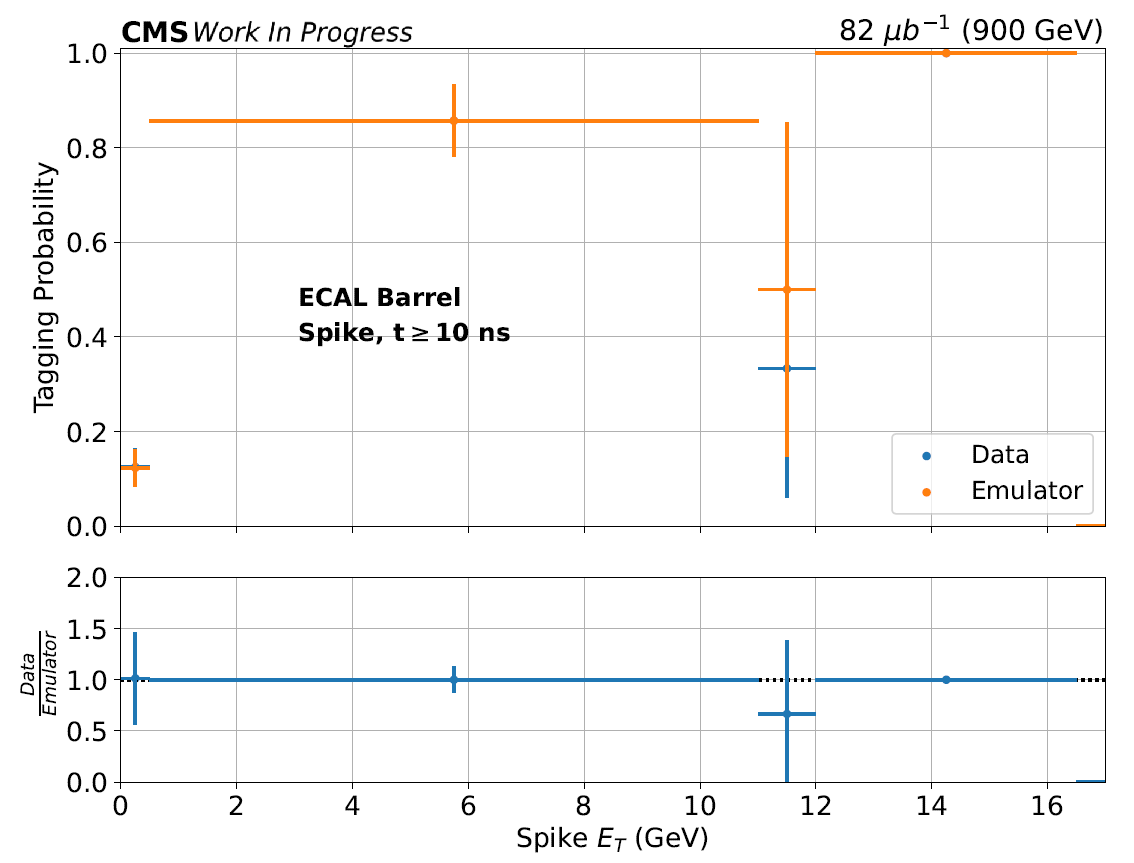
\includegraphics[width=.475\textwidth]{Images/ECAL/DW/2021Collisions_Sev_four_VeryLate_DataOverEmulatorTaggingProbability_linear.png}}%
    \hfill
    \subfloat[2022 collisions, $\delta_{min}$ = 2.5 GeV working point]{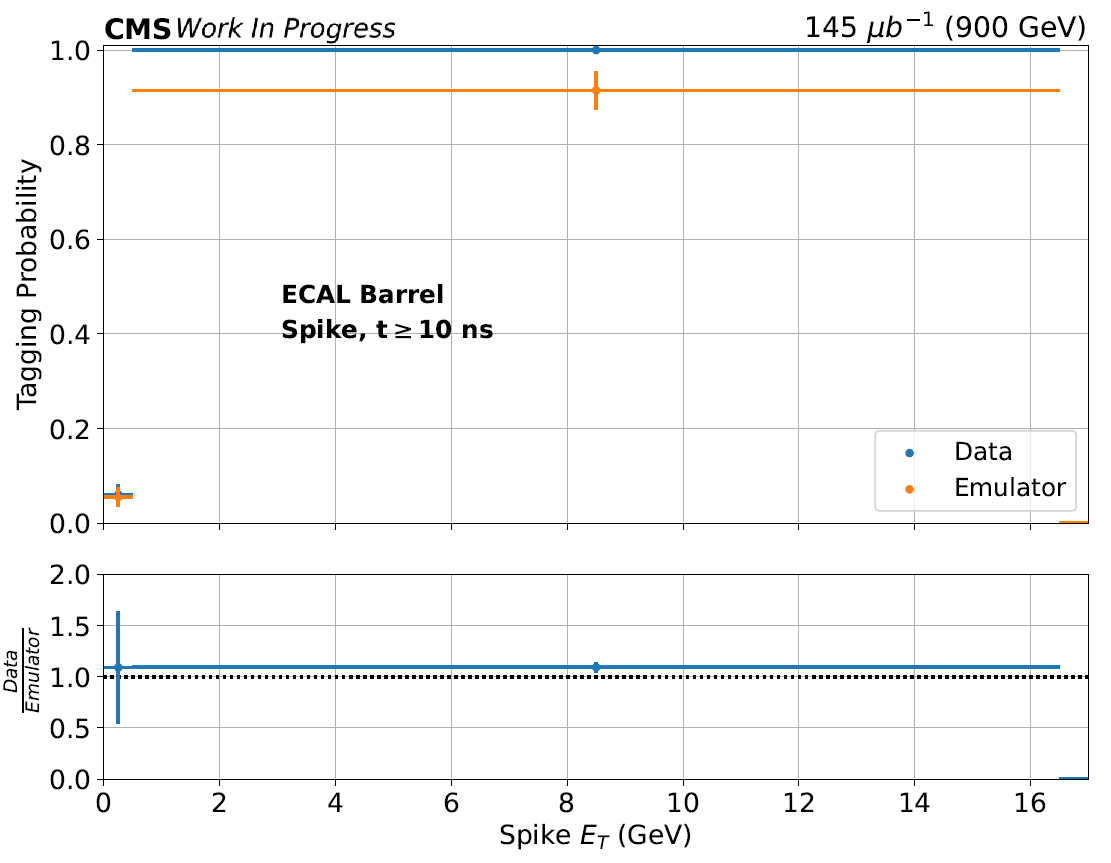
\includegraphics[width=.475\textwidth]{Images/ECAL/DW/2022Collisions_Sev_four_VeryLate_DataOverEmulatorTaggingProbability_linear.png}}%
    \caption{Tagging probability in data and as computed by the emulator for Severity 4 matched TPs with offline matched reconstructed times $>$ 10 ns. \label{fig:SevFourDataEmulatorTagging}}%
\end{figure}  

For the in time severity zero matched TP cases shown in Figure \ref{fig:SevZeroDataEmulatorTagging}, the tagging probabilities as evaluated by the data and emulator are in agreement within 0.6\%. This indicates that for the most part, the emulator can be trusted for accurately estimating the performance of the double weights mechanism on in-time severity zero matched TPs when re-emulating CMS data. 

For the late severity four matched TP cases shown in Figure \ref{fig:SevFourDataEmulatorTagging}, in the 2021 data sample there is one TP with disagreement in data and emulator energy in the 11 GeV bin. This individual TP requires further investigation to understand if this disagreement is due to the double weights mechanism or not. Apart from this TP, the double weights tagging probability as determined by data and the emulator are in agreement within 1.4\%, and fully in agreement for highly energetic TPs. In the 2022 data, there are a number of TPs which different data and emulated energies, which may or may not change the tagging probabilities computed in the data and emulator, which disagree by about 10\%. These differences require further investigation: They may be found to be due to the double weights in which the algorithm or weight values may need to be updated, or there may be an issue in the emulator which would need to be fixed.

Finally, during 2022 the LHC provided further beam splashes to CMS. The ECAL operations teams took this opportunity to run with double weights in ``killing $+$ tagging" mode, in which ECAL strips which have a greater ODD amplotide than EVEN amplitude have their energy zeroed (killing), and if there is a large amount of zeroing in a given ECAL TP, a flag is set (tagging). The functionality of this configuration was tested as it may be a potentially useful mode to use in the future, for instance to have the information of which regions of ECAL have their energy at least partially killed by double weights. An event from a 2022 beam splash running with ECAL double weights in killing $+$ tagging mode is shown in Figure \ref{fig:2022_BeamSplash_DWTagging}. 

\begin{figure}[H]%
    \setcounter{subfigure}{0}
    \centering
    \subfloat[TP energy distribution]{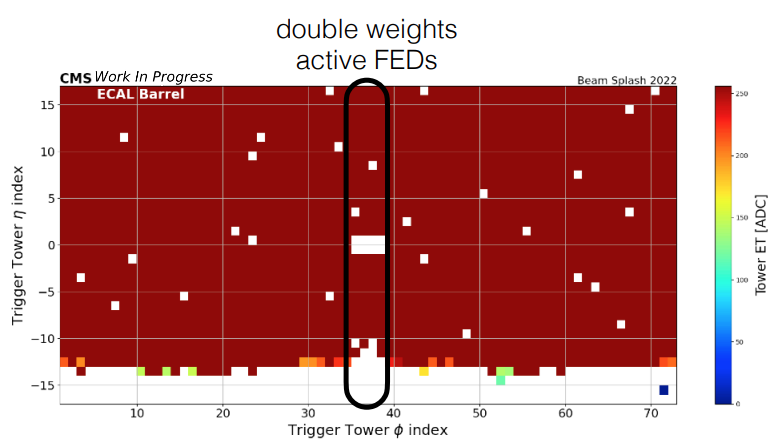
\includegraphics[width=.475\textwidth]{Images/ECAL/DW/BeamSplash2022_DW_TagNKill_Energy.png}}%
    %\hfill
    \subfloat[TPs tagged as out of time]{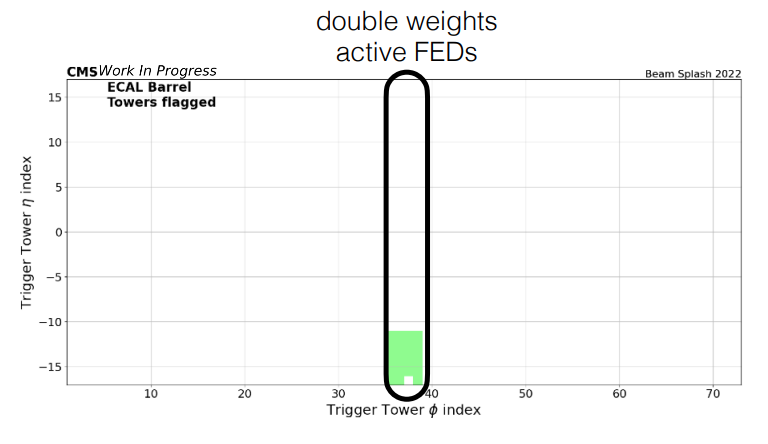
\includegraphics[width=.475\textwidth]{Images/ECAL/DW/BeamSplash2022_DW_TagNKill_Tagging.png}}%
    \caption{ECAL TP energies and TPs tagged as out-of-time by double weights in killing $+$ tagging mode during a 2022 CMS beam splash. \label{fig:2022_BeamSplash_DWTagging}}%
\end{figure} 

In this configuration, the majority of the ECAL barrel ran with its nominal Run 2 configuration, but killing $+$ tagging mode was set for two supermodules in the center of the detector. In one supermodule in which negatively out-of-time signals are expected, it is observed that there is some amount of killing of energy as the energy in that region is lower than the other supermodules with similar TP times, as the particle from the splash propagate from -$\eta$ to $+\eta$ and are expected to have roughly the same timing per $\eta$ index, and it can be seen that TPs in the same region are tagged. This is the first instance of ECAL running with double weights in killing $+$ tagging mode, and shows that this previously untested configuration appears to work as expected. 

While these initial re-emulation and data checks with double weights show potential gain at the ECAL TP level, as high energy spikes are tagged and removed while there is a minimal impact on low in-time signals and the emulator appears to provide an accurate representation of the double weights mechanism applied to in time signal-like TPs, the next necessary thing to check is the impact of double weights on CMS L1 quantities. This includes the effect on L1 rates, and L1 turn-on curves. A potential gain would be a decrease in the L1 rates due to the removal of spikes, which may allow for a lowering of the L1 seed energy thresholds. This would potentially allow for the collection of more Higgs pair production events in electromagnetic final states, including HH$\rightarrow$WW$\gamma\gamma$, which may improve the sensitivity of this and other Higgs pair production analyses to be performed at CMS using the LHC Run 3 dataset. 